\documentclass[12pt,oneside, a4paper]{book}

\usepackage{etex}
\usepackage{xcolor}
\usepackage[pdftex]{graphicx}
\usepackage{rotating}
\usepackage{epsfig}
\usepackage{epstopdf}
\usepackage{cmap}
\usepackage[T1]{fontenc}
\usepackage[utf8]{inputenc}
\usepackage[english,croatian]{babel}
\usepackage[unicode,hidelinks]{hyperref}
\hypersetup{
  pdftitle={Utjecaj transkodiranja na kvalitetu VoIP poziva},
  pdfauthor={Ahmed Softić},
  pdfsubject={Završni rad -- VoIP transkodiranje},
  pdfkeywords={VoIP, transkodiranje, FreeSWITCH, PESQ, STOI, RTP}
}
\usepackage{mathptmx}
\usepackage{amscd}
\usepackage{amssymb}
\usepackage{amsmath}
\usepackage{amsfonts}
\usepackage[left=2.5cm,right=2.5cm,top=2.5cm,bottom=2.5cm]{geometry}
\usepackage{setspace} 
\usepackage{hhline}
\usepackage{enumerate}
\usepackage{delarray}
\usepackage{array}  
\usepackage{tabularx} 
\usepackage{multirow}  
\usepackage{float}
\usepackage{placeins}
\usepackage[bf, font=small]{caption}
\usepackage[labelfont=small, font=small]{subcaption}
\usepackage{wasysym}
\usepackage{subeqnarray}
\usepackage{pdflscape} % prikaz stranice u položenom formatu
\usepackage{enumitem} % postavke nabrajanja
\usepackage[toc,page]{appendix}
\newcommand{\HRule}{\rule{\linewidth}{0.5mm}}
\usepackage{makeidx}
\usepackage{nomencl}
\usepackage{listings}
\lstset{basicstyle=\ttfamily,breaklines=true}
\usepackage{courier}
\usepackage{tikz}
\usetikzlibrary{arrows}
\usepackage{fancyhdr} 
\setlength{\headheight}{16pt}

\fancypagestyle{plain}{%
  \fancyhf{}% brisanje zaglavlja i podnožja
  \fancyfoot[OR]{{\thepage}}%
  \fancyfoot[EL]{{\thepage}}%
  \renewcommand{\headrulewidth}{0pt}%
}

% Postavke indeksa; za unos pojma koristi se \index{pojam}.
%\usepackage{makeidx}
%\makeindex
% Postavke popisa oznaka; za unos se koristi \nomenclature{oznaka}{opis}.
%\usepackage{nomencl}
%\makenomenclature
%\renewcommand{\nomname}{Popis oznaka}



\linespread{1.3}
\setlist{nolistsep}   % sažeto nabrajanje
\renewcommand{\thefootnote}{\fnsymbol{footnote}}  

\let\savenumberline\numberline
\def\numberline#1{\savenumberline{#1.}}

\pagestyle{fancyplain}

%\rfoot{\thepage}
\AtBeginDocument{\addtocontents{toc}{\protect\thispagestyle{empty}}}
\AtBeginDocument{\addtocontents{lof}{\protect\thispagestyle{empty}}}
\AtBeginDocument{\addtocontents{lot}{\protect\thispagestyle{empty}}}

%\rhead{\slshape \nouppercase \leftmark}
%\lhead{} %delete left header


%Podesavanje izgleda referenci
\usepackage[square, numbers, sort]{natbib} 

%Promjena naziva pojedinih poglavlja sa Hrvatskog na Bosanski
% Naziv bibliografije mijenja se u „Literatura“.
\addto\captionscroatian{%
  \renewcommand{\bibname}{Literatura}
  \renewcommand{\tablename}{Tabela}
  \renewcommand{\nomname}{Popis oznaka}
  \renewcommand{\indexname}{Indeks pojmova}
  \renewcommand{\lstlistingname}{Program}
}
%"Popis tablica" u "Popis tabela"
\addto\captionscroatian{\renewcommand{\listtablename}{Popis tabela}}
\addto\captionscroatian{\renewcommand\appendixname{Prilog}}
\addto\captionscroatian{\renewcommand\appendixpagename{Prilozi}}
\renewcommand\appendixtocname{Prilozi}

% Rezultati se generišu iz results/summary/results_summary.csv.
% Automatski generisano; ne uređivati ručno.
% Izvor: results/summary/results_summary.csv
\newcommand{\BrojKonfiguracija}{25}
\newcommand{\BrojPoziva}{250}
\newcommand{\PassthroughPESQ}{4{,}242}
\newcommand{\TranscodePESQ}{3{,}401}
\newcommand{\RazlikaPESQ}{0{,}841}
\newcommand{\PassthroughPESQEnglish}{4.242}
\newcommand{\TranscodePESQEnglish}{3.401}
\newcommand{\RazlikaPESQEnglish}{0.841}
\newcommand{\RelativnaRazlikaPESQ}{19{,}8\%}
\newcommand{\PassthroughCPU}{2{,}0\%}
\newcommand{\TranscodeCPU}{3{,}9\%}
\newcommand{\OmjerCPU}{2{,}0}
\newcommand{\DeltaT}{5{,}98}
\newcommand{\DeltaDF}{19}
\newcommand{\DeltaP}{0{,}000009}
\newcommand{\RazlikaCIDonja}{0{,}547}
\newcommand{\RazlikaCIGornja}{1{,}136}
\newcommand{\HedgesG}{1{,}28}
\newcommand{\ProsjekPremaPCMU}{3{,}815}
\newcommand{\ProsjekPremaPCMA}{3{,}713}
\newcommand{\ProsjekPremaGSevenTwoTwo}{3{,}214}
\newcommand{\ProsjekPremaOpusu}{3{,}867}
\newcommand{\ProsjekPremaGSMu}{2{,}396}


%\usepackage{etoolbox}
%\patchcmd{\chapter}{\thispagestyle{plain}}{\thispagestyle{fancyplain}}{}{}


\begin{document}

\hypersetup{pageanchor=false}

\frontmatter

%%%%%%%%%%%%%%%%%%%% NASLOVNA STRANA %%%%%%%%%%%%%%%%%%%%%%%%
\begin{titlepage}
\begin{center}

% \includegraphics[width=0.25\textwidth]{etf-logo.png}~\\[0.1cm]
% Dodati službeni logo tek nakon preuzimanja fakultetskog predloška.
\textsc{\Large Univerzitet u Sarajevu}\\[0.2cm]  
\textsc{\Large Elektrotehnički fakultet}\\[0.2cm] 
\textsc{\Large Odsjek za računarstvo i informatiku}\\[3cm]\HRule \\[0.5cm] 
{\huge \bfseries Utjecaj transkodiranja na kvalitetu VoIP poziva} \\[0.4cm] 
\HRule \\[0.5cm]

\textsc{\Large Završni rad}\\[0.4cm]
\textsc{\Large - Prvi ciklus studija - }\\[1.5cm]

% Student i mentor
\textbf{ 
\Large Student:\\  
\Large Ahmed Softić\\[1cm]  
\Large Mentor: \\[0.2cm] 
\Large prof. dr Saša Mrdović} 
\vfill

% Dno naslovne stranice
{\large Sarajevo, \\august 2026.}

\end{center} 
\end{titlepage}
\hypersetup{pageanchor=true}

% Sažetak, postavka rada i izjava o autentičnosti nalaze se u odvojenim datotekama.

\chapter*{Sažetak}
\addcontentsline{toc}{chapter}{Sažetak}

U radu se ispituje utjecaj transkodiranja na govorni signal u VoIP pozivu koji prolazi kroz \mbox{FreeSWITCH} SIP server u ulozi B2BUA uređaja. Transkodiranje je potrebno kada krajnji uređaji koriste različite audio-kodeke, pa server mora u stvarnom vremenu dekodirati signal kodiran izvornim kodekom i ponovo ga kodirati u odredišni format.

Razvijena je metodologija zasnovana na analizi PCAP zapisa mrežnog saobraćaja. Iz RTP paketa izdvajaju se signal ulaznog kanala A (engl. \emph{A-leg}) i signal izlaznog kanala B (engl. \emph{B-leg}), dekodiraju se u PCM format, vremenski poravnavaju i porede metrikama PESQ MOS-LQO i STOI. Primarno poređenje mjeri dodatnu promjenu između dva kanala poziva, dok dodatno poređenje originalnog WAV-a i B-lega pokazuje krajnju očuvanost signala.

Ispitana je puna matrica od \BrojKonfiguracija{} usmjerenih kombinacija pet kodeka (PCMU, PCMA, G.722, GSM i Opus), sa po deset ponavljanja, odnosno ukupno \BrojPoziva{} poziva. U primarnoj analizi prosječni PESQ MOS-LQO po konfiguraciji iznosio je \PassthroughPESQ{} za prijenos bez transkodiranja i \TranscodePESQ{} za transkodiranje, uz prosječnu dodatnu degradaciju od \RazlikaPESQ{} boda. U end-to-end analizi odgovarajući grupni prosjeci iznose 3,170 i 2,608, a dodatna degradacija prema kontroli istog izvornog kodeka 0,563 boda. Najveći dodatni gubici zabilježeni su pri kodiranju u GSM. Kodiranje u Opus uglavnom bolje čuva ulazni signal, uz veću potrošnju procesora, ali ne može vratiti sadržaj izgubljen u prethodnom uskopojasnom kodeku. Rezultati važe za kontrolisano lokalno okruženje bez namjerno uvedenih mrežnih smetnji.

\textbf{Ključne riječi:} VoIP, transkodiranje, FreeSWITCH, PESQ, STOI, RTP, audio-kodeci, kvaliteta govora

\chapter*{Abstract}
\addcontentsline{toc}{chapter}{Abstract}
\begin{otherlanguage}{english}

This thesis examines the effect of transcoding on the speech signal in a Voice over IP call routed through a FreeSWITCH server acting as a back-to-back user agent. A reproducible method based on packet-capture analysis was developed. The incoming A-leg and outgoing B-leg RTP streams are extracted, decoded, time-aligned, and compared using PESQ MOS-LQO and STOI. The primary comparison measures the additional change introduced between the server legs, while a supplementary comparison of the original waveform and the B-leg measures end-to-end signal preservation.

The complete directed matrix of \BrojKonfiguracija{} configurations formed by five codecs (PCMU, PCMA, G.722, GSM, and Opus) was evaluated with ten repetitions per configuration, for a total of \BrojPoziva{} calls. In the primary analysis, the mean PESQ MOS-LQO was \PassthroughPESQEnglish{} without transcoding and \TranscodePESQEnglish{} with transcoding; the mean additional degradation relative to the matching source-codec baseline was \RazlikaPESQEnglish{} points. In the supplementary end-to-end analysis, the corresponding group means were 3.170 and 2.608, with an additional degradation of 0.563 points. Encoding to GSM produced the largest losses. Encoding to Opus generally preserved the incoming signal better at the cost of higher processor usage, but could not restore information previously removed by a narrowband codec. The conclusions apply to the controlled local environment without intentionally introduced network impairments.

\textbf{Keywords:} VoIP, transcoding, FreeSWITCH, PESQ, STOI, RTP, audio codecs, speech quality
\end{otherlanguage}


%%%%%%%%%%%%%%%%%%%% POSTAVKA RADA %%%%%%%%%%%%%%%%%%%%%%%%%%%%%%%
\thispagestyle{empty} % skip pagination
\begin{center}
\textbf{\LARGE POSTAVKA RADA}
\end{center}

\vspace{1cm}

\textbf{Tema:} Utjecaj transkodiranja na kvalitetu VoIP poziva

\vspace{0.5cm}

\textbf{Student:} Ahmed Softić

\vspace{0.5cm}

\textbf{Mentor:} prof.\ dr\ Saša Mrdović

\vspace{1cm}

\textbf{Opis zadatka:}

\begin{enumerate}
\item Proučiti osnovne koncepte VoIP tehnologije s naglaskom na audio-kodeke i njihovu ulogu u kvalitetu poziva
\item Analizirati proces transkodiranja u VoIP sistemima i identifikovati scenarije kada je transkodiranje neophodno
\item Uspostaviti eksperimentalno okruženje zasnovano na platformi FreeSWITCH koje omogućava kontrolisano ispitivanje različitih kombinacija kodeka
\item Razviti metodologiju zasnovanu na analizi PCAP zapisa za mjerenje promjene govornog signala između ulaza i izlaza medijskog poslužitelja
\item Implementirati automatizovane skripte za izdvajanje govornog signala iz RTP paketa u PCAP datotekama i dekodiranje izvornih formata kodeka
\item Izvršiti mjerenja objektivnih metrika kvaliteta (PESQ i STOI) i procesorskog opterećenja za odabrane kombinacije kodeka
\item Analizirati rezultate i identifikovati kompromise između kvaliteta, kompatibilnosti i potrošnje resursa
\item Donijeti preporuke za konfiguraciju VoIP sistema sa aspekta optimizacije kvaliteta i resursa
\end{enumerate}

\vspace{1cm}

\noindent Sarajevo, april 2025.

\vspace{2cm}

\hfill\begin{minipage}{6cm}
\centering
\rule{6cm}{0.4pt}\\
prof.\ dr\ Saša Mrdović\\
Mentor
\end{minipage}


%%%%%%%%%%%%%%%%%%%% IZJAVA AUTORA %%%%%%%%%%%%%%%%%%%%
\thispagestyle{empty}

\vspace*{8cm}

\section*{Izjava o autentičnosti}

Izjavljujem da je ovaj rad moj autorski rad i da sam ga samostalno izradio koristeći navedenu literaturu i konsultacije sa mentorom. Svi citati i parafrazirani dijelovi rada pravilno su označeni i referencirani.

\vspace{3cm}

\hfill\begin{minipage}{6cm}
\centering
\rule{6cm}{0.4pt}\\
Ahmed Softić
\end{minipage}


%%%%%%%%%%%%%%%%%%%%% SADRŽAJ %%%%%%%%%%%%%%%%%%%%%%%%%
%\clearpage
\tableofcontents

%%%%%%%%%%%%%%% POPIS SLIKA %%%%%%%%%%%%%%%%%%%%%%%%%%%
%\clearpage
\listoffigures
\addcontentsline{toc}{chapter}{Popis slika}

%%%%%%%%%%%%%%% POPIS TABELA %%%%%%%%%%%%%%%%%%%%%%%%%%
%\clearpage
\listoftables
\addcontentsline{toc}{chapter}{Popis tabela}

%%%%%%%%%%%%%%% POPIS OZNAKA %%%%%%%%%%%%%%%%%%%%%%%%%%%
\cleardoublepage % početak nove stranice
\pagestyle{fancyplain} % ponovno uključivanje zaglavlja i podnožja
\fancyhf{}
\lhead{\nouppercase{\fancyplain{}{\leftmark}}}
\renewcommand{\chaptermark}[1]{\markboth{#1}{}}
\renewcommand{\footrulewidth}{0.4pt} % linija podnožja
\rfoot{\thepage}
\cfoot{}

%%%%%%%%%%%%%%%%%%%%%%%%%%%%%%%%%%%%%%%%%%%%%%%%%%%%%%%%%%%%%%%%%%%%
\mainmatter

%%%%%%%%%%%%%%%%%%%%%%%%%%%%%%%%%%%%%%%%%%%%%%%%%%%%%%%%%%%%%%%%%%%%
%%%%%%%%%%%%%%%%%%%%%%%%% POGLAVLJA %%%%%%%%%%%%%%%%%%%%%%%%%%%%%%%%
%%%%%%%%%%%%%%%%%%%%%%%%%%%%%%%%%%%%%%%%%%%%%%%%%%%%%%%%%%%%%%%%%%%%

% Poglavlja se nalaze u odvojenim datotekama.
\chapter{Uvod}
\label{ch:uvod}

VoIP (engl. \emph{Voice over Internet Protocol}) je tehnologija koja omogućava prijenos poziva u obliku mrežnih paketa umjesto putem namjenskih kanala klasične telefonije. Uspostavljanje poziva, pregovaranje medijskih parametara i prijenos govora obavljaju različiti, međusobno povezani protokoli. SIP upravlja uspostavljanjem sesije, SDP opisuje ponuđene medije i kodeke, a RTP prenosi kodirani govor. Takav pristup olakšava integraciju komunikacijskih usluga, ali kvalitet razgovora čini zavisnim od mrežnih uslova, izbora kodeka i obrade medijskog toka.

\section{Motivacija i problem}

U VoIP sistemima različiti uređaji i gatewayi često ne podržavaju iste audio-kodeke. Ako krajnji uređaji pri uspostavljanju poziva ne dogovore zajednički kodek, medijski server mora dekodirati ulazni signal i ponovo ga kodirati u format koji podržava drugi učesnik. Ovaj postupak omogućava interoperabilnost, ali može izazvati izobličenje govornog signala i dodatno kašnjenje. Transkodiranje također troši procesorske resurse medijskog servera.

Iako su karakteristike pojedinačnih kodeka dobro dokumentovane, praktičan utjecaj njihove konverzije zavisi od implementacije, smjera konverzije i frekvencije uzorkovanja. Zbog toga je korisno posmatrati stvarni RTP tok prije i poslije obrade u medijskom serveru, a ne samo izolovane programske kodere~\cite{tandem-encoding}.

\section{Cilj i istraživačka pitanja}

Cilj ovog rada je izmjeriti degradaciju govornog signala i procesorsko opterećenje nastalo pri transkodiranju na medijskom serveru FreeSWITCH. Porede se scenariji bez transkodiranja, u kojima oba krajnja uređaja koriste isti kodek, sa scenarijima transkodiranja, u kojima uređaji koriste različite kodeke pa server mora pretvoriti signal iz jednog formata u drugi. Analizirana je puna matrica od \BrojKonfiguracija{} kombinacija kodeka PCMU, PCMA, G.722, GSM i Opus, sa po deset ponavljanja.

Istraživanje daje odgovor na četiri pitanja: koliku degradaciju transkodiranje uvodi u izlazni govorni signal u odnosu na ulazni signal, kako smjer konverzije i izbor kodeka utječu na rezultat, koliko procesorskih resursa zahtijeva transkodiranje te koliko se konačni audiosignal razlikuje od originala.

\section{Metodologija}

FreeSWITCH ima ugrađenu mogućnost snimanja poziva, ali se takav snimak formira iz internog PCM signala. Zbog toga ne obuhvata završno kodiranje i paketizaciju izlaznog RTP toka te nije prikladan za mjerenje cjelokupne promjene između ulaznog i izlaznog kraka.

RTP paketi analizirani u ovom radu snimljeni su na mrežnom interfejsu alatom tshark. Njihov korisni sadržaj zadržava format dogovorenog kodeka, nakon čega se dekodira u PCM, rekonstruira prema RTP vremenskim oznakama i vremenski poravnava. Poređenjem signala ulaznog kraka A i izlaznog kraka B izdvaja se dodatna degradacija između dva kraka FreeSWITCH poziva. Dopunsko poređenje koristi originalni WAV kao referencu i izlazni signal kraka B kao degradirani signal, čime obuhvata cijeli put od izvornog zapisa do izlaza servera. Uz PESQ MOS-LQO i STOI mjeri se i ukupna potrošnja procesora FreeSWITCH servera tokom poziva.

\section{Struktura rada}

Rad je organizovan u osam poglavlja. U Poglavlju~\ref{ch:uvod} predstavljeni su motivacija, problem, cilj, istraživačka pitanja i primijenjena metodologija. Poglavlje~\ref{ch:osnove-voip} detaljno prolazi kroz osnove VoIP poziva, od SIP signalizacije i SDP pregovaranja do RTP prijenosa govornih paketa. Poglavlje~\ref{ch:kodeci} objašnjava uzorkovanje, kvantizaciju, paketizaciju i matematičke osnove korištenih kodeka. Na toj osnovi Poglavlje~\ref{ch:transkodiranje} opisuje postupak pretvaranja iz jednog kodeka u drugi, moguće gubitke i dva nivoa mjerenja. Poglavlje~\ref{ch:kvaliteta} uvodi korištene metrike te njihovo objašnjenje i pozadinu. Poglavlje~\ref{ch:eksperiment} dokumentuje eksperimentalno okruženje, vremensko poravnanje uzoraka, obradu podataka i statistički postupak. Poglavlje~\ref{ch:rezultati} prikazuje serverske i end-to-end rezultate, nakon čega Poglavlje~\ref{ch:zakljucak} daje sažetak nalaza, ograničenja i preporuke.

\chapter{VoIP komunikacija: SIP, SDP i RTP}
\label{ch:osnove-voip}

VoIP (engl. \emph{Voice over Internet Protocol}) je komunikacijska tehnologija koja omogućava prijenos govora u obliku mrežnih paketa putem IP mreža. Za razliku od tradicionalne telefonije, koja se uglavnom zasniva na komutaciji namjenskih kanala u PSTN mreži (engl. \emph{Public Switched Telephone Network}), VoIP koristi paketni prijenos putem privatnih IP mreža ili javnog interneta. Govor se digitalizira, kodira, pakuje i prenosi zajedničkom mrežnom infrastrukturom. Za uspostavljanje poziva VoIP se oslanja na SIP. U okviru uspostavljanja sesije SDP opisuje ponuđene medijske parametre, a nakon dogovora kodirani govor prenosi se RTP-om.


\section{Funkcionalni dijelovi VoIP sistema}

Tipičan VoIP sistem sadrži krajnje SIP uređaje (engl. \emph{endpoints}), signalizacijske servere i, prema potrebi, medijske servere. Krajnji uređaj može biti IP telefon, softverski telefon ili aplikacija ugrađena u drugi sistem. SIP proxy usmjerava signalizacijske zahtjeve, registrar čuva vezu između SIP adrese korisnika i njegove trenutne mrežne lokacije, dok lokacijski servis pomaže pri pronalaženju odredišta~\cite{rfc3261}.

Medijski gateway povezuje različite mreže ili medijske formate. B2BUA (engl. \emph{Back-to-Back User Agent}) nalazi se između dva SIP endpointa i uspostavlja dva odvojena dijaloga: jedan prema endpointu A, a drugi prema endpointu B. Time dobija veću kontrolu nad signalizacijom i može nezavisno pregovarati kodeke na dva kraka poziva. Ako medijski tok prolazi kroz B2BUA, uređaj može obrađivati govorni signal, uključujući njegovo transkodiranje.

Ovakva arhitektura može se posmatrati kroz dvije sfere:

\begin{itemize}
    \item \textbf{signalizacija} određuje ko učestvuje u pozivu, koje su mogućnosti strana i kada sesija počinje ili završava;
    \item \textbf{medijski prijenos} prenosi kodirani govor nakon što su dogovoreni adrese, portovi i formati.
\end{itemize}

\noindent SIP i SDP pripadaju signalizacijskom dijelu, ali SDP određuje parametre budućeg RTP toka. Zbog toga odluka donesena tokom signalizacije određuje način obrade medijskog sadržaja tokom razgovora.

\section{SIP adresiranje, poruke i dijalozi}

SIP (engl. \emph{Session Initiation Protocol}) je tekstualni aplikacijski protokol za uspostavljanje, izmjenu i prekid multimedijskih sesija~\cite{rfc3261}. Korisnik se identifikuje SIP URI-jem, odnosno adresom oblika \texttt{sip:korisnik@domena}. URI predstavlja logički identitet korisnika. Stvarna IP adresa i port mogu se mijenjati, pa uređaj porukom REGISTER obavještava registrar na kojoj je mrežnoj lokaciji trenutno dostupan.

SIP zahtjev sadrži početni red, zaglavlja i, po potrebi, tijelo poruke. Najvažnije metode u osnovnom glasovnom pozivu su:

\begin{itemize}
    \item \texttt{REGISTER} prijavljuje trenutnu lokaciju korisnika;
    \item \texttt{INVITE} pokreće sesiju i najčešće prenosi SDP ponudu;
    \item \texttt{ACK} potvrđuje konačni uspješni odgovor na INVITE;
    \item \texttt{BYE} završava već uspostavljeni poziv;
    \item \texttt{CANCEL} zaustavlja zahtjev prije uspostavljanja sesije;
    \item \texttt{OPTIONS} ispituje mogućnosti udaljenog SIP entiteta bez uspostavljanja poziva.
\end{itemize}

Odgovori se označavaju trocifrenim kodovima i dijele u šest klasa:

\begin{itemize}
    \item \texttt{1xx} označava privremene odgovore, na primjer \texttt{100 Trying} ili \texttt{180 Ringing};
    \item \texttt{2xx} označava uspješno izvršenu akciju;
    \item \texttt{3xx} služi za preusmjeravanje;
    \item \texttt{4xx} predstavlja grešku u korisničkom zahtjevu;
    \item \texttt{5xx} predstavlja serversku grešku;
    \item \texttt{6xx} služi za globalne greške.
\end{itemize}

Zaglavlja \texttt{Call-ID}, \texttt{From} i \texttt{To} te redni broj \texttt{CSeq} omogućavaju koreliranje poruka u transakcije i dijaloge. Zaglavlje \texttt{Via} sadrži informacije o putu IP transporta zahtjeva te služi da tom rutom bude transportovan odgovor, a \texttt{Contact} daje adresu za naredne zahtjeve unutar dijaloga.

SIP transakcija obuhvata jedan zahtjev i odgovore na njega, dok dijalog predstavlja dugotrajniji odnos između dva SIP endpointa. Poziv uspostavljen metodom INVITE zato sadrži više transakcija: početni INVITE, kasniji BYE i, prema potrebi, dodatne zahtjeve za promjenu sesije. Endpointi mogu razmjenjivati i informacije metodom INFO. Ovo razlikovanje je važno jer SIP dijalog može ostati aktivan dok se parametri medija mijenjaju novom SDP razmjenom.

SIP poruke mogu se prenositi UDP-om, TCP-om ili drugim transportom. Kada se koristi UDP, pouzdanost signalizacije ostvaruje sam SIP retransmisijom poruka prema pravilima transakcije i pripadajućim vremenskim brojačima~\cite{rfc3261}. Osnovni RTP protokol ne garantuje isporuku i sam ne zahtijeva ponovno slanje izgubljenih paketa. Odvojeno dogovoreni RTP mehanizmi mogu u pojedinim sistemima omogućiti retransmisiju~\cite{rfc4588}. Moderna VoIP tehnologija u nekim slučajevima podržava retransmisiju RTP paketa, dok prijemnik koristi buffering i dejitter kako bi ublažio posljedice promjenjivih mrežnih uslova. Signalizacija i medijski prijenos zato imaju različita pravila pouzdanosti i vremenske zahtjeve. Gubitak SIP poruke može odgoditi ili onemogućiti uspostavljanje sesije, dok gubitak RTP paketa u uspostavljenoj sesiji stvara kratki prekid ili aktivira prikrivanje gubitka u dekoderu.

SIP dijalog određuju tri vrijednosti: globalno jedinstveni \texttt{Call-ID}, lokalni \texttt{tag} i udaljeni \texttt{tag}~\cite{rfc3261}. B2BUA ne prosljeđuje samo isti dijalog, nego prema svakoj strani djeluje kao zaseban korisnički agent. Zbog toga kanali A i B mogu imati različite identifikatore, redne brojeve poruka i mrežne adrese. Ova osobina omogućava FreeSWITCH-u da nezavisno pregovara kodeke, ali ujedno znači da se stanje oba dijaloga i oba medijska toka mora održavati tokom cijelog poziva.

\section{Uspostavljanje i završetak poziva}

Pojednostavljen tok uspješnog poziva prikazan je na Slici~\ref{fig:sip-call-flow}. Registracija nije prikazana jer je odvojena od samog dijaloga. Pozivatelj šalje INVITE s opisom ponuđenih medijskih atributa. Nakon privremenih odgovora, pozvana strana u odgovoru \texttt{200 OK} prihvata sesiju i vraća vlastiti SDP. Poruka ACK dovršava trosmjernu razmjenu, nakon čega se audio prenosi RTP-om. BYE i završni \texttt{200 OK} prekidaju sesiju.

B2BUA mijenja poruke i održava zasebne identifikatore dijaloga, SDP opise i RTP parametre na dva kanala. Zato kodeci prihvaćeni na kanalima A i B ne moraju biti isti.

\begin{figure}[htbp]
\centering
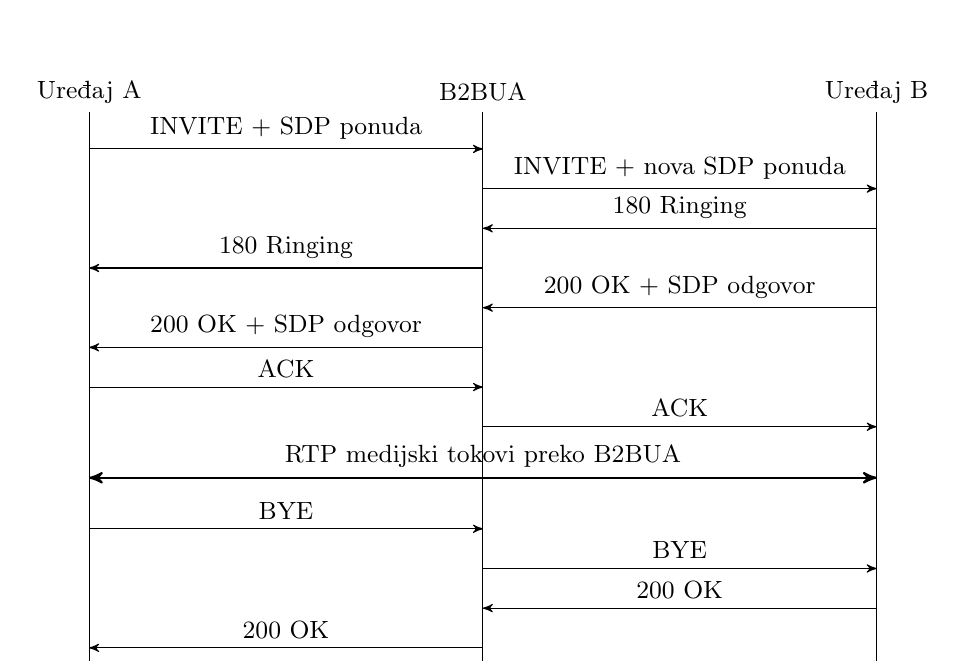
\begin{tikzpicture}[x=1cm,y=0.72cm,>=stealth',font=\small]
    \node (a) at (0,0) {Uređaj A};
    \node (fs) at (5,0) {B2BUA};
    \node (b) at (10,0) {Uređaj B};
    \draw (0,-0.35) -- (0,-10.3);
    \draw (5,-0.35) -- (5,-10.3);
    \draw (10,-0.35) -- (10,-10.3);
    \draw[->] (0,-1) -- node[above]{INVITE + SDP ponuda} (5,-1);
    \draw[->] (5,-1.7) -- node[above]{INVITE + nova SDP ponuda} (10,-1.7);
    \draw[->] (10,-2.4) -- node[above]{180 Ringing} (5,-2.4);
    \draw[->] (5,-3.1) -- node[above]{180 Ringing} (0,-3.1);
    \draw[->] (10,-3.8) -- node[above]{200 OK + SDP odgovor} (5,-3.8);
    \draw[->] (5,-4.5) -- node[above]{200 OK + SDP odgovor} (0,-4.5);
    \draw[->] (0,-5.2) -- node[above]{ACK} (5,-5.2);
    \draw[->] (5,-5.9) -- node[above]{ACK} (10,-5.9);
    \draw[<->,thick] (0,-6.8) -- node[above]{RTP medijski tokovi preko B2BUA} (10,-6.8);
    \draw[->] (0,-7.7) -- node[above]{BYE} (5,-7.7);
    \draw[->] (5,-8.4) -- node[above]{BYE} (10,-8.4);
    \draw[->] (10,-9.1) -- node[above]{200 OK} (5,-9.1);
    \draw[->] (5,-9.8) -- node[above]{200 OK} (0,-9.8);
\end{tikzpicture}
\caption{Pojednostavljen tok SIP poziva preko B2BUA uređaja}
\label{fig:sip-call-flow}
\end{figure}

\section{SDP opis i pregovaranje medija}

SDP (engl. \emph{Session Description Protocol}) nije transportni protokol i sam ne šalje audio. To je tekstualni opis sesije koji se obično nalazi u tijelu SIP poruke. Sadrži vrstu medija, mrežnu adresu, port, RTP profil, oznake formata i njihove parametre~\cite{rfc4566}. Pravila modela ponude i odgovora određuju kako dvije strane usaglašavaju kompatibilan skup parametara~\cite{rfc3264}. SIP endpoint može ponuditi više kodeka i medijskih opisa, ali mora biti sposoban primiti medij u svakom ponuđenom formatu. Redoslijed formata predstavlja prioritet pošiljaoca i utječe na izbor kodeka.

Pojednostavljen SDP primjer može izgledati ovako:

\begin{lstlisting}
v=0
o=userA 3747 3747 IN IP4 192.0.2.10
s=VoIP call
c=IN IP4 192.0.2.10
t=0 0
m=audio 4000 RTP/AVP 111 9 0 8 3
a=rtpmap:111 opus/48000/2
a=fmtp:111 maxaveragebitrate=30000;useinbandfec=0
a=rtpmap:9 G722/8000
a=rtpmap:0 PCMU/8000
a=rtpmap:8 PCMA/8000
a=rtpmap:3 GSM/8000
a=ptime:20
\end{lstlisting}

Red \texttt{m=audio} nudi UDP port 4000, RTP profil i poredanu listu vrsta korisnog sadržaja (engl. \emph{payload type}, PT). Atribut \texttt{a=rtpmap} povezuje PT vrijednost s nazivom kodeka, RTP frekvencijom sata i brojem kanala. \texttt{a=fmtp} prenosi parametre specifične za format, dok \texttt{a=ptime} predlaže trajanje zvuka u jednom paketu. Statičke vrijednosti kao što su PT 0 za PCMU, 8 za PCMA, 9 za G.722 i 3 za GSM definisane su RTP profilom~\cite{rfc3551}; Opus koristi dinamičku vrijednost iz raspona 96--127~\cite{rfc7587}.

Odgovor ne smije proizvoljno izabrati kodek koji nije ponuđen. Prihvaćeni medijski tok mora odgovarati ponuđenom formatu i dogovorenim parametrima. Redoslijed u ponudi iskazuje prioritet pošiljaoca, ali konačan izbor zavisi i od sposobnosti i politike druge strane. Kod B2BUA arhitekture postoje dvije odvojene razmjene ponude i odgovora. Ako je na prvom kraku prihvaćen PCMU, a na drugom Opus, signalizacija je uspješno uspostavila poziv, ali je istovremeno stvorila potrebu za transkodiranjem iz PCMU u Opus, kao i u suprotnom smjeru.

Tabela~\ref{tab:sdp-two-legs} prikazuje logiku takvog slučaja. Izbor kodeka nije jedna zajednička odluka za cijeli poziv, nego dvije odluke koje B2BUA povezuje. Presjek mogućnosti na svakom pojedinačnom kanalu dovoljan je da se taj kanal uspostavi; jednak kodek na oba kraka potreban je tek ako se želi izbjeći transkodiranje. U takvim slučajevima moguće je koristiti direktni medijski tok (engl. \emph{media bypass}), pri kojem B2BUA ostaje u signalizacijskom putu, dok uređaji A i B razmjenjuju RTP pakete direktno.

\begin{table}[htbp]
\centering
\caption{Primjer odvojenog pregovaranja medija na dva kanala B2BUA poziva}
\label{tab:sdp-two-legs}
\small
\begin{tabularx}{\textwidth}{|l|X|X|}
\hline
\textbf{Element} & \textbf{Kanal A} & \textbf{Kanal B} \\
\hline
Mogućnosti krajnjeg uređaja & PCMU, PCMA & Opus, G.722 \\
Ponuda koju obrađuje B2BUA & PCMU, PCMA, G.722 & Opus, G.722, PCMU \\
Prihvaćeni format & PCMU/8000 & Opus/48000/2 \\
RTP vremenska osnova & 8000 otkucaja/s & 48000 otkucaja/s \\
Posljedica & \multicolumn{2}{c|}{dekodiranje PCMU, promjena PCM toka i kodiranje u Opus} \\
\hline
\end{tabularx}
\end{table}

SDP također opisuje smjer medijskog toka pomoću četiri atributa:

\begin{itemize}
    \item \texttt{sendrecv} dozvoljava slanje i prijem medijskog sadržaja;
    \item \texttt{sendonly} dozvoljava samo slanje medijskog sadržaja;
    \item \texttt{recvonly} dozvoljava samo prijem medijskog sadržaja;
    \item \texttt{inactive} privremeno isključuje oba smjera medijskog toka.
\end{itemize}

Novi pregovori mogu se obaviti unutar postojećeg dijaloga metodom UPDATE ili novim INVITE zahtjevom, odnosno re-INVITE postupkom~\cite{rfc3261,rfc3311}. Njima se mogu promijeniti port, skup kodeka, smjer ili drugi važni medijski parametri. Primjer ovog ponašanja se javlja u Call Centrima kada je business use case da se poziv stavi na čekanje ili spoji na drugog agenta. U praktičnom dijelu ovog rada parametri ostaju nepromijenjeni tokom aktivnog dijaloga.

\section{RTP i RTCP prijenos govora}

Nakon dogovora, govor se najčešće prenosi protokolom RTP preko UDP-a~\cite{rfc3550}. RTP ne garantuje isporuku niti ponovno šalje izgubljene pakete jer bi zakašnjeli paketi često bili manje korisni od propuštenog paketa. Umjesto toga, zaglavlje svakog RTP paketa nosi podatke potrebne primaocu:

\begin{itemize}
    \item \textbf{redni broj} raste za svaki paket i omogućava otkrivanje gubitka i promjene redoslijeda;
    \item \textbf{vremenska oznaka} opisuje položaj prvog uzorka korisnog sadržaja u medijskom vremenu i omogućava reprodukciju pravilnim ritmom;
    \item \textbf{PT vrijednost} označava način tumačenja korisnog sadržaja prema SDP dogovoru;
    \item \textbf{SSRC} razlikuje izvor sinhronizacije unutar RTP sesije.
\end{itemize}

RTP frekvencija sata nije uvijek jednaka stvarnoj frekvenciji dekodiranog PCM signala. Posebno, G.722 u standardnom RTP profilu koristi sat od 8 kHz zbog historijske kompatibilnosti, iako kodek obrađuje širokopojasni signal uzorkovan na 16 kHz~\cite{rfc3551}. Opus u RTP-u uvijek koristi sat od 48 kHz, nezavisno od trenutno kodiranog audio-opsega~\cite{rfc7587}.

Za pakete koji nose jednako trajanje zvuka očekivani prirast vremenske oznake je

\begin{equation}
\Delta t_{RTP}=f_{RTP}T_p,
\end{equation}

gdje je $f_{RTP}$ frekvencija RTP sata, a $T_p$ trajanje zvuka u paketu. Za 20 ms dobijaju se prirasti 160 pri satu od 8 kHz i 960 pri satu od 48 kHz. Redni broj govori da li paket nedostaje, a vremenska oznaka koliko medijskog vremena treba proteći između dva korisna sadržaja. Te dvije informacije nisu zamjenjive: paket može stići urednim rednim brojem, ali nakon namjerne pauze u RTP vremenskoj liniji.

Varijacija vremena dolaska paketa naziva se kolebanje kašnjenja (engl. jitter). RTP prijemnik procjenjuje jitter iz promjene relativnog tranzitnog vremena uzastopnih paketa, odnosno iz razlike između njihovog razmaka pri slanju i razmaka pri dolasku~\cite{rfc3550}:

\begin{equation}
J_i=J_{i-1}+\frac{|D_{i-1,i}|-J_{i-1}}{16},
\end{equation}

gdje $D_{i-1,i}$ opisuje promjenu razlike između vremena slanja i dolaska. Veći jitter zahtijeva veći međuspremnik (engl. buffer), a veći međuspremnik dodaje kašnjenje. Premalen međuspremnik odbacuje pakete koji stignu nakon roka reprodukcije. Kvalitet VoIP-a zato nije određen samo vjernošću kodeka nego i ravnotežom između kontinuiteta reprodukcije i kašnjenja paketa.

Primalac koristi međuspremnik kašnjenja (engl. \emph{jitter buffer}) da ublaži nejednaka vremena dolaska paketa. RTCP periodično šalje izvještaje o broju primljenih i izgubljenih paketa, kašnjenju i vremenskoj vezi izvora. RTCP ne prenosi sam govor i ne popravlja automatski gubitke, ali daje podatke za praćenje kvaliteta sesije.

U lokalnom eksperimentu nisu namjerno uvedeni gubitak paketa, promjena redoslijeda ni dodatni jitter. Time su posmatrane razlike prvenstveno povezane s kodecima i obradom na serveru. Takva postavka ipak ne simulira javnu mrežu. U stvarnim uslovima rezultat zavisi i od prikrivanja gubitka paketa, veličine buffera, kašnjenja te eventualne redundantnosti ili FEC mehanizma.

\section{Od SIP dogovora do transkodiranja}

Cijeli put može se sumirati na sljedeći način: SIP pronalazi učesnika i upravlja dijalogom. SDP na svakom kanalu opisuje dostupne kodeke i mrežne parametre. Izabrani kodek određuje sadržaj RTP paketa, a medijski server povezuje dva kanala. Kada su odabrani formati jednaki, moguće je proslijediti medij bez ponovnog kodiranja. Kada se razlikuju, server mora dekodirati jedan format i kodirati drugi. Za razumijevanje posljedica te operacije potrebno je prvo objasniti kako se govor digitalizuje i koje informacije pojedini kodeci čuvaju ili odbacuju.

\chapter{Digitalizacija govora i VoIP kodeci}
\label{ch:kodeci}

U procesu pregovora medijskih atributa uz pomoć SDP-a bira se način na koji će se govorni signal prenositi u RTP paketima. Kodek ne označava samo format datoteke ili mrežnu oznaku, nego skup pravila za uzorkovanje, kvantizaciju, uklanjanje redundantnosti i rekonstrukciju zvuka. Razlike između tih pravila određuju potrebnu propusnost, frekvencijski opseg, računarsku kompleksnost i vrstu degradacije koja se može pojaviti pri transkodiranju.

\section{Od analognog govora do niza uzoraka}

Mikrofon pretvara zvučne signale u kontinuirani električni signal $x_a(t)$. Analogno-digitalni pretvarač najprije ograničava njegov frekvencijski opseg filterom, a zatim uzima vrijednosti u jednakim vremenskim razmacima. Diskretni signal definisan je izrazom

\begin{equation}
x[n]=x_a(nT_s), \qquad T_s=\frac{1}{f_s},
\end{equation}

gdje je $f_s$ frekvencija uzorkovanja izražena u hercima, a $T_s$ period između dva uzorka. Jedan herc znači jedan ciklus u sekundi, dok vrijednost 8000 uzoraka u sekundi znači da se amplituda signala mjeri svakih 125~$\mu$s. Uzorkovanje i frekvencija zvuka povezani su, ali nisu ista veličina: ton od 1000 Hz opisuje hiljadu perioda zvučnog talasa u sekundi, a uzorkovanje od 8000 Hz opisuje osam hiljada mjerenja njegove amplitude.

Prema Nyquistovom kriteriju, za rekonstrukciju signala čija je najviša frekvencija $f_{max}$ potrebno je~\cite{oppenheim-schafer}

\begin{equation}
f_s > 2f_{max}.
\end{equation}

Zbog toga sistem uzorkovan na 8 kHz može predstavljati frekvencije samo do 4 kHz, uz praktični zaštitni pojas analognog filtera. Tradicionalni telefonski govor prenosi približno 300--3400 Hz i naziva se uskopojasnim (engl. \emph{narrowband}). Širokopojasni govor (engl. \emph{wideband}) proširuje korisni opseg približno do 7 kHz i obično koristi 16 kHz uzorkovanje. Opus dodatno podržava superširokopojasni i punopojasni rad, do približno 20 kHz audio-opsega pri 48 kHz uzorkovanju~\cite{rfc6716}.

Veća frekvencija uzorkovanja ne znači sama po sebi da signal sadrži više korisne informacije. Povećanje signala sa 8 na 48 kHz interpolacijom dodaje uzorke, ali ne može obnoviti frekvencije koje je prethodno uklonio uskopojasni koder. Ova činjenica kasnije postaje važna za razumijevanje asimetrije smjerova transkodiranja.

Ako se prije uzorkovanja ne uklone komponente iznad polovine frekvencije uzorkovanja, one se preslikavaju u niži dio spektra. Za sinus frekvencije $f$ uzorkovan frekvencijom $f_s$, uzorci se ne mogu razlikovati od komponente na frekvenciji $|f-kf_s|$ za odgovarajući cijeli broj $k$. Ova pojava naziva se aliasing i nakon uzorkovanja se ne može pouzdano poništiti. Ulazni anti-alias filter i filter prije smanjenja frekvencije uzorkovanja zato nisu samo implementacijski detalji, nego dio očuvanja kvaliteta.

Pojmovi uskopojasni, širokopojasni i punopojasni opisuju sačuvani audio-opseg, a ne samo broj uzoraka. Njihova veza prikazana je u Tabeli~\ref{tab:audio-bandwidth}. Granice su približne jer stvarni prijenosni opseg zavisi od filtera i kodeka.

\begin{table}[htbp]
\centering
\caption{Veza audio-opsega i tipične frekvencije uzorkovanja}
\label{tab:audio-bandwidth}
\small
\begin{tabular}{|l|c|c|l|}
\hline
\textbf{Naziv opsega} & \textbf{Tipični audio-opseg} & \textbf{$f_s$} & \textbf{Primjer} \\
\hline
Uskopojasni & približno 300--3400 Hz & 8 kHz & G.711, GSM FR \\
Širokopojasni & približno 50--7000 Hz & 16 kHz & G.722 \\
Superširokopojasni & približno do 14 kHz & 32 kHz & Opus \\
Punopojasni & približno do 20 kHz & 48 kHz & Opus \\
\hline
\end{tabular}
\end{table}

\section{Kvantizacija, PCM i brzina prijenosa}

Uzorak je nakon mjerenja još uvijek vrijednost iz gotovo kontinuiranog raspona amplituda. Kvantizator ga preslikava na jedan od $L=2^N$ nivoa, gdje je $N$ broj bita po uzorku. Za ravnomjernu kvantizaciju raspona od $x_{min}$ do $x_{max}$ korak je~\cite{gray-neuhoff}

\begin{equation}
\Delta=\frac{x_{max}-x_{min}}{2^N},
\end{equation}

a kvantizacijska greška idealno ostaje unutar približno $-\Delta/2$ i $\Delta/2$. Za sinusni signal pune amplitude približni odnos signal-kvantizacijski šum raste za oko 6 dB po dodatnom bitu. Ta aproksimacija objašnjava korist veće rezolucije, ali nije mjera perceptivnog kvaliteta govora.

Ako se greška ravnomjernog kvantizatora približno posmatra kao slučajna veličina ravnomjerno raspoređena u tom intervalu, njena snaga je

\begin{equation}
\sigma_q^2=\frac{\Delta^2}{12}.
\end{equation}

Za sinus pune amplitude slijedi poznata aproksimacija $SQNR\approx6{,}02N+1{,}76$ dB. Stvarni govor nema stalnu punu amplitudu niti je kvantizacijska greška uvijek nezavisna od signala, pa izraz služi za objašnjenje odnosa rezolucije i greške, a ne za predviđanje PESQ rezultata. Perceptivni kodeci dodatno raspoređuju grešku prema vremenskim i frekvencijskim osobinama sluha.

PCM (engl. \emph{Pulse Code Modulation}) predstavlja svaki kvantizirani uzorak njegovom binarnom oznakom. Za $C$ kanala, frekvenciju uzorkovanja $f_s$ i $N$ bita po uzorku nekomprimirana brzina iznosi

\begin{equation}
R_{PCM}=f_sNC.
\end{equation}

Naprimjer, monofoni linearni PCM na 8 kHz sa 16 bita zahtijeva 128 kbit/s. G.711 prenosi osmobitne sažete i kvantizirane uzorke i zato zahtijeva 64 kbit/s. Kodeci s manjom brzinom ne zapisuju svaki uzorak nezavisno, nego iskorištavaju statističku i perceptivnu redundantnost govora.

\subsection{Kompandovanje}

Govor često ima mnogo uzoraka male amplitude i manji broj uzoraka velike amplitude. Ravnomjerna osmobitna kvantizacija svim dijelovima raspona daje jednak korak, pa je relativna greška posebno nepovoljna za tihe dijelove. Kompandovanje (engl. compressing + expanding) prije kvantizacije nelinearno proširuje male, a sabija velike amplitude. Za normalizirani ulaz $|x|\leq1$, $\mu$-law koristi funkciju

\begin{equation}
F_{\mu}(x)=\operatorname{sgn}(x)
\frac{\ln(1+\mu|x|)}{\ln(1+\mu)}, \qquad \mu=255,
\end{equation}

dok A-law koristi parcijalno definisanu karakteristiku

\begin{equation}
F_A(x)=\operatorname{sgn}(x)
\begin{cases}
\dfrac{A|x|}{1+\ln A}, & 0\leq |x|<\dfrac{1}{A},\\[6pt]
\dfrac{1+\ln(A|x|)}{1+\ln A}, & \dfrac{1}{A}\leq |x|\leq1,
\end{cases}
\qquad A\approx87{,}6.
\end{equation}

Primalac primjenjuje inverznu funkciju i dobija aproksimaciju originalne amplitude. PCMU i PCMA zato predstavljaju sličan signal, ali njihove osmobitne kodne riječi i kvantizacijski nivoi nisu jednaki~\cite{g711}.

\section{Okviri, paketi i stvarna mrežna propusnost}

Kodek obrađuje uzorke u okvirima određenog trajanja. Ako paket obuhvata $T_p$ sekundi zvuka, broj uzoraka po kanalu je

\begin{equation}
N_p=f_sT_p.
\end{equation}

Pri trajanju od 20 ms, uskopojasni signal na 8 kHz ima 160 uzoraka, a signal na 48 kHz 960 uzoraka. Kraći paketi smanjuju vrijeme čekanja da se okvir popuni, ali povećavaju broj zaglavlja u sekundi. Duži paketi smanjuju relativni mrežni trošak, ali povećavaju paketizacijsko kašnjenje i količinu govora izgubljenu gubitkom jednog paketa.

Brzina kodeka nije jednaka ukupnoj brzini na mreži. Za IPv4 bez dodatnih opcija svaki RTP/UDP/IP paket nosi 12+8+20=40 bajtova zaglavlja. G.711 s 20 ms zvuka šalje 160 bajtova korisnog sadržaja 50 puta u sekundi, pa bez zaglavlja sloja veze zahtijeva

\begin{equation}
R_{\mathrm{mreza}}=50\,(160+40)\,8=80\ \text{kbit/s}.
\end{equation}

Kodek manje nominalne brzine zato štedi korisni sadržaj, ali dio protokolskih zaglavlja postaje veći. Ethernet, VLAN, tuneliranje, šifriranje i druga zaglavlja dodatno povećavaju stvarnu propusnost.

Za kodek brzine $R_c$, trajanje paketa $T_p$ i ukupno $H$ bajtova zaglavlja po paketu, približna IP brzina može se izraziti kao

\begin{equation}
R_{IP}=R_c+\frac{8H}{T_p}.
\end{equation}

Pri istih 40 bajtova RTP/UDP/IPv4 zaglavlja i 20 ms paketizacije samo zaglavlja dodaju 16 kbit/s. To je četvrtina korisne brzine G.711, ali više od nominalne brzine GSM Full Rate kodeka. Agregiranje više okvira kodeka u paket smanjuje ovaj dodatak, uz cijenu većeg paketizacijskog kašnjenja i većeg vremenskog gubitka kada jedan paket izostane.

\section{Kodeci obuhvaćeni eksperimentom}

\subsection{G.711: PCMU i PCMA}

G.711 je talasni kodek koji uzorkuje govor na 8 kHz i svaki uzorak predstavlja jednom osmobitnom kompandiranom vrijednošću~\cite{g711}. PCMU primjenjuje $\mu$-law, tradicionalno zastupljen u Sjevernoj Americi i Japanu, dok PCMA primjenjuje A-law, uobičajen u evropskim telefonskim mrežama. Obje varijante rade pri 64 kbit/s, imaju malu algoritamsku složenost i malo kašnjenje. Njihov nedostatak su veća propusnost u odnosu na govorne kodeke niske brzine i uskopojasni audio-opseg.

Pretvaranje PCMU$\leftrightarrow$PCMA ne zahtijeva promjenu frekvencije uzorkovanja. Ipak, dekodirana amplituda mora se ponovo preslikati na drugačiji skup kvantizacijskih nivoa, pa višestruka konverzija nije matematički identična izvornom nizu kodnih riječi.

\subsection{G.722}

G.722 je širokopojasni kodek za audio-opseg približno do 7 kHz. Ulaz uzorkovan na 16 kHz dijeli se kvadraturnim ogledalskim filterima u niži i viši podpojas. Svaki podpojas zatim koristi adaptivnu diferencijalnu impulsno-kodnu modulaciju (ADPCM)~\cite{g722}. Umjesto pune amplitude, ADPCM kvantizira razliku između trenutnog uzorka i vrijednosti koju prediktor očekuje:

\begin{equation}
e[n]=x[n]-\widehat{x}[n].
\end{equation}

Ako je predikcija dobra, $e[n]$ ima manji dinamički raspon od $x[n]$ i može se predstaviti manjim brojem bita. Adaptacija prediktora i kvantizatora prati promjene signala. Režim korišten u radu ima 64 kbit/s, ali daje širi frekvencijski opseg od G.711 pri istoj nominalnoj brzini. Njegova RTP frekvencija sata iz historijskih razloga ostaje 8 kHz, iako je dekodirani audio na 16 kHz~\cite{rfc3551}.

\subsection{GSM Full Rate}

GSM 06.10 Full Rate napravljen je za mobilnu telefoniju i znatno manju brzinu od G.711. Svakih 20 ms, odnosno 160 uzoraka na 8 kHz, predstavlja sa 260 bita, što daje 13 kbit/s~\cite{etsi-gsm-fr}. Kodek pripada porodici RPE-LTP (engl. \emph{Regular Pulse Excitation--Long Term Prediction}).

Kratkoročna linearna predikcija modelira trenutni govorni uzorak kombinacijom prethodnih uzoraka:

\begin{equation}
\widehat{s}[n]=\sum_{k=1}^{p}a_k s[n-k], \qquad e[n]=s[n]-\widehat{s}[n].
\end{equation}

Koeficijenti $a_k$ opisuju kratkotrajni oblik vokalnog trakta, a rezidual $e[n]$ sadrži ono što prediktor nije objasnio. Dugoročna predikcija iskorištava periodičnost zvučnih glasova, dok pravilno raspoređeni pobudni impulsi aproksimiraju preostali signal. Prenose se parametri modela, a ne svaki uzorak. Time se ostvaruje velika ušteda propusnosti, ali greška modeliranja i kvantizacija parametara mogu stvoriti prepoznatljive govorne artefakte, naročito nakon ponovnog kodiranja.

\subsection{Opus}

Opus je otvoreni kodek projektovan za interaktivni govor i opći zvuk, s brzinama od približno 6 do 510 kbit/s i okvirima od 2,5 do 60 ms~\cite{rfc6716}, te kombinuje dva pristupa: SILK koristi linearnu predikciju prilagođenu govoru, dok CELT koristi transformacijsko kodiranje zasnovano na modificiranoj diskretnoj kosinusnoj transformaciji. U hibridnom režimu SILK kodira niži, a CELT viši dio spektra.

Transformacijski koder blok vremenskih uzoraka predstavlja koeficijentima frekvencijskih područja. Raspoloživi broj bitova može se raspodijeliti područjima važnijim za percepciju, dok se manje važni detalji grublje kvantiziraju. Opus može mijenjati bitrate, audio-opseg i unutrašnji način rada bez promjene naziva RTP formata. U SDP-u se uvijek oglašava s RTP satom od 48 kHz i dva kanala u oznaci \texttt{opus/48000/2}, čak i kada aplikacija prenosi mono govor~\cite{rfc7587}.

Fleksibilnost Opusa omogućava dobar odnos kvaliteta i propusnosti, ali koder i dekoder imaju veću računarsku složenost od jednostavnog G.711 preslikavanja. U ovom eksperimentu korišten je konstantni režim do 30 kbit/s, monofoni signal i paketi od 20 ms.

\section{Uporedne karakteristike}

Tabela~\ref{tab:codec-overview} sumira osobine bitne za ovaj rad. Frekvencija PCM-a označava brzinu dekodiranog signala korištenu u obradi; RTP sat je mrežna vremenska osnova i kod G.722 nije jednak toj vrijednosti.

\begin{table}[htbp]
\centering
\caption{Osnovne karakteristike ispitanih kodeka}
\label{tab:codec-overview}
\small
\begin{tabularx}{\textwidth}{|l|c|c|c|X|}
\hline
\textbf{Kodek} & \textbf{PCM} & \textbf{RTP sat} & \textbf{Brzina} & \textbf{Osnovni postupak} \\
\hline
PCMU & 8 kHz & 8 kHz & 64 kbit/s & PCM s $\mu$-law kompandovanjem \\
PCMA & 8 kHz & 8 kHz & 64 kbit/s & PCM s A-law kompandovanjem \\
G.722 & 16 kHz & 8 kHz & 64 kbit/s & podpojasni ADPCM \\
GSM & 8 kHz & 8 kHz & 13 kbit/s & RPE-LTP govorni model \\
Opus & 48 kHz & 48 kHz & promjenjiva & SILK, CELT ili hibridni režim \\
\hline
\end{tabularx}
\end{table}

Kodeke nije ispravno rangirati samo prema frekvenciji uzorkovanja ili nominalnoj brzini. Kvalitet zavisi od sadržaja, bitratea, implementacije, broja uzastopnih kodiranja i mrežnih uslova. Za predmet ovog rada posebno je važno da svaki kodek u zajednički PCM međusignal donosi vlastita ograničenja. Transkoder može promijeniti format i broj uzoraka, ali ne može vratiti detalje koje je prethodna faza nepovratno odbacila.

\chapter{Transkodiranje u VoIP sistemima}
\label{ch:transkodiranje}

Transkodiranje je pretvaranje medijskog sadržaja iz formata jednog kodeka u format drugog. Potrebno je kada dvije strane mogu uspostaviti SIP sesiju, ali na svojim medijskim kanalima koriste različite kodeke. Signalizacija omogućava uspostavljanje poziva između dvije strane. Medijski server zatim u stvarnom vremenu pretvara audio iz jednog kodeka u drugi.

\section{Mjesta i razlozi nastanka transkodiranja}

Transkodiranje se javlja na granici mreža s različitim pravilima, između tradicionalne i IP telefonije, u SBC uređajima (engl. \emph{Session Border Controller}), medijskim gateway-ima, konferencijskim sistemima, sistemima za snimanje i B2BUA platformama. Razlozi nisu samo tehnička nepodudarnost krajnjih uređaja. Operator može namjerno izabrati kodek manje brzine na ograničenoj vezi, širokopojasni kodek unutar lokalne mreže ili format koji zahtijeva vanjski pružalac usluge.

U idealnom slučaju oba kanala dogovaraju isti kodek i poslužitelj može proslijediti kodirane okvire bez dekodiranja i ponovnog kodiranja. Takav način rada često se naziva prolazom medija (engl. \emph{passthrough}). Isti naziv kodeka ipak nije dovoljan: moraju biti kompatibilni i parametri kao što su trajanje okvira, broj kanala i posebne postavke kodeka. Ako formati nisu kompatibilni, audio se mora dekodirati i ponovo kodirati. Isto vrijedi kada server obrađuje PCM signal radi konferencije, snimanja ili drugog DSP postupka.

\section{Tok obrade u medijskom poslužitelju}

Za smjer A$\rightarrow$B, RTP korisni sadržaj prvo dekodira dekoder kodeka A. Dobijeni PCM signal može se vremenski prilagoditi te mu se mogu promijeniti broj kanala i frekvencija uzorkovanja. Koder B zatim ga pretvara u niz kodiranih okvira. Poslužitelj tim okvirima dodjeljuje novi RTP redni broj, vremensku oznaku i SSRC odgovarajućeg izlaznog toka. Pojednostavljeni tok ove obrade prikazan je na Slici~\ref{fig:transcode-pipeline}.

\begin{figure}[htbp]
\centering
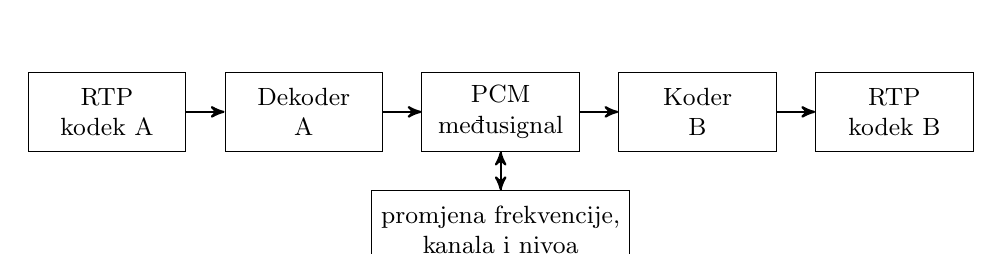
\begin{tikzpicture}[node distance=1.8cm, auto, >=stealth',
    block/.style={rectangle, draw, minimum height=1cm, minimum width=2cm, align=center, font=\small},
    arrow/.style={->, thick}]
    \node[block] (rtp1) {RTP\\kodek A};
    \node[block, right of=rtp1, node distance=2.5cm] (dec) {Dekoder\\A};
    \node[block, right of=dec, node distance=2.5cm] (pcm) {PCM\\međusignal};
    \node[block, right of=pcm, node distance=2.5cm] (enc) {Koder\\B};
    \node[block, right of=enc, node distance=2.5cm] (rtp2) {RTP\\kodek B};
    \node[block, below of=pcm, node distance=1.5cm] (dsp) {promjena frekvencije,\\kanala i nivoa};

    \draw[arrow] (rtp1) -- (dec);
    \draw[arrow] (dec) -- (pcm);
    \draw[arrow] (pcm) -- (enc);
    \draw[arrow] (enc) -- (rtp2);
    \draw[arrow] (pcm) -- (dsp);
    \draw[arrow] (dsp) -- (pcm);
\end{tikzpicture}
\caption{Pojednostavljeni tok transkodiranja kodeka A u kodek B}
\label{fig:transcode-pipeline}
\end{figure}

Ako su $D_A$ i $E_B$ dekoder i koder, a $R_{A,B}$ potrebna obrada PCM-a, izlaz se može zapisati kao

\begin{equation}
y_B=E_B\!\left(R_{A,B}\!\left(D_A(p_A)\right)\right),
\end{equation}

gdje je $p_A$ ulazni kodirani sadržaj. Obrnuti smjer glasi

\begin{equation}
y_A=E_A\!\left(R_{B,A}\!\left(D_B(p_B)\right)\right).
\end{equation}

Redoslijed ovih operacija utječe na rezultat. U smjerovima A$\rightarrow$B i B$\rightarrow$A razlikuju se ulazni signal, završni koder i često način promjene frekvencije uzorkovanja. Zato se rezultat jednog smjera ne može koristiti kao rezultat obrnutog smjera.

Važno je razlikovati transkodiranje od samog prepakivanja. Prepakivanje zadržava kodirani korisni sadržaj, ali mu mijenja transportni ili kontejnerski wrapper. Ono ne uvodi novu kvantizaciju kodeka. Pri transkodiranju signal se najčešće prvo dekodira, a zatim kodira u drugi format. Time se mijenja način predstavljanja audio sadržaja. U eksperimentu se izraz \emph{bez transkodiranja} koristi za jednake kodeke na oba kanala, dok provjera RTP okvira pokazuje koliko FreeSWITCH može očuvati ili proslijediti postojeći sadržaj.

\section{Promjena frekvencije uzorkovanja}

Kada kodeci rade na različitim frekvencijama, PCM međusignal mora proći konverziju. Smanjenje sa $f_{s1}$ na $f_{s2}$ zahtijeva niskopropusni filtar prije odbacivanja uzoraka, kako se frekvencije iznad nove Nyquistove granice ne bi preslikale u niži dio spektra. Pojednostavljeno, za cjelobrojni faktor $M$ izlaz nakon filtriranja $h[k]$ može se zapisati kao

\begin{equation}
y[m]=\sum_k x[k]h[mM-k].
\end{equation}

Povećanje frekvencije dodaje nove položaje uzoraka i interpolacijskim filtrom procjenjuje njihove vrijednosti. Ono daje format s većim brojem uzoraka, ali ne stvara autentičan visokofrekvencijski sadržaj. Naprimjer, GSM$\rightarrow$Opus može proizvesti PCM na 48 kHz, ali govor ostaje ograničen informacijom koju je GSM prethodno sačuvao ispod približno 4 kHz. Nasuprot tome, Opus$\rightarrow$GSM mora trajno odbaciti viši dio spektra. Smjerovi zato imaju različito fizičko značenje čak i prije primjene završnog kodera.

Kada se frekvencija uzorkovanja mijenja u odnosu $L/M$, resampler najprije povećava broj uzoraka faktorom $L$. Signal se zatim filtrira, nakon čega se zadržava svaki $M$-ti uzorak~\cite{oppenheim-schafer}. Postupak se može zapisati kao

\begin{equation}
y[m]=\sum_{n=-\infty}^{\infty}x[n]h[mM-nL],
\end{equation}

gdje $h$ predstavlja interpolacijski niskopropusni filtar. Kvalitet resampliranja zavisi od širine prijelaznog područja, potiskivanja zaustavnog opsega i numeričke preciznosti. Oštriji filter (brže prelazi iz propusnog u nepropusni opseg) bolje ograničava aliasing, ali zahtijeva više operacija i može povećati kašnjenje. U lancu s više promjena frekvencije poželjno je izbjeći nepotrebne uzastopne konverzije.

\section{Izvori gubitaka i degradacije}

\subsection{Ponovljena kvantizacija}

Svaki kodek s gubicima preslikava veliki skup mogućih ulaza na manji skup kodnih reprezentacija. Nakon dekodiranja dobija se aproksimacija, a ne original. Novo kodiranje tu aproksimaciju ponovo kvantizira. Greške pojedinih faza nisu nužno nezavisne niti se jednostavno sabiraju, jer sljedeći koder analizira signal koji već sadrži artefakte prethodnog kodera.

Kod PCMU$\leftrightarrow$PCMA riječ je uglavnom o ponovljenom nelinearnom kvantiziranju amplitude. Kod GSM-a i Opusa mogu se dodatno kvantizirati parametri modela govora ili transformacijski koeficijenti. Rezultat može biti ujednačavanje signala, promjena kratkotrajne energije, tonalni artefakti ili slabije očuvanje prijelaza između glasova.

\subsection{Tandemsko kodiranje}

Uzastopni spoj dekoder--koder naziva se tandemskim kodiranjem. Ako je originalni signal $s$, a par kodeka $E_A,D_A$ zatim $E_B,D_B$, krajnji signal je

\begin{equation}
\widehat{s}=D_B\!\left(E_B\!\left(D_A\!\left(E_A(s)\right)\right)\right).
\end{equation}

Čak i kada svaki pojedinačni kodek daje prihvatljiv rezultat, njihov tandem može pojačati artefakte ili odbaciti različite dijelove informacije. Ranija istraživanja VoIP kvaliteta zato izdvajaju višestruko kodiranje kao poseban faktor, uz mrežni gubitak i kašnjenje~\cite{tandem-encoding,sun-voip-models}.

\subsection{Ograničenje frekvencijskog opsega}

Najmanji sačuvani opseg u lancu postavlja gornju granicu onoga što se kasnije može rekonstruisati. Kada širokopojasni signal prođe kroz uskopojasni kodek, frekvencije iznad njegovog propusnog područja nepovratno nestaju. Naknadno kodiranje u G.722 ili Opus ne vraća ih. Zbog toga se visoka izmjerena sličnost nakon uskopojasnog izvora mora tumačiti kao malo dodatno oštećenje već ograničenog signala, a ne kao dokaz širokopojasnog krajnjeg kvaliteta.

\subsection{Paketizacija i vremenska obrada}

Kodeci mogu koristiti različite veličine okvira i određeni broj narednih uzoraka za obradu, što se naziva \emph{look-ahead}. Takva obrada uvodi dodatno algoritamsko kašnjenje. Poslužitelj ponekad mora prikupiti dovoljno uzoraka prije formiranja izlaznog okvira. Bufferi, promjena veličine paketa i resampling dodaju kašnjenje nezavisno od mrežnog puta. U ovom radu se signali vremenski poravnavaju prije poređenja, pa rezultat kvaliteta ne predstavlja mjeru razgovornog kašnjenja.

Ukupno jednosmjerno kašnjenje može se rastaviti na više doprinosa:

\begin{equation}
d_{uk}=d_{pak}+d_{alg,A}+d_{obr}+d_{alg,B}+d_{mre\check{z}a}+d_{jitter},
\end{equation}

U izrazu $d_{pak}$ označava vrijeme paketizacije, $d_{alg}$ algoritamsko kašnjenje kodeka, a $d_{obr}$ vrijeme obrade u serveru. Posljednja dva člana predstavljaju kašnjenje mrežnog prijenosa i jitter buffera. Transkodiranje neposredno povećava obradu i uvodi algoritamske komponente oba kodeka. PESQ nakon vremenskog poravnanja može pokazati visoku vjernost i kada je razgovorno kašnjenje neprihvatljivo, zbog čega se kvaliteta signala i interaktivnost moraju razmatrati odvojeno~\cite{itu-g114}.

\section{Dva komplementarna nivoa mjerenja}

Učinak transkodiranja može se posmatrati iz dvije referentne tačke. Ako se izlazni B-leg usporedi s ulaznim A-legom, početno kodiranje kodekom A zajedničko je objema stranama usporedbe. Dobijena razlika prvenstveno opisuje ono što su dodali medijski poslužitelj, promjena frekvencije i odredišni koder. Ovaj nivo je pogodan za pitanje: koliko je FreeSWITCH dodatno promijenio signal koji je primio?

Ako se isti B-leg usporedi s originalnim WAV signalom koji je reproducirao uređaj A, mjera obuhvata i početno kodiranje kodekom A. Ona odgovara drugom pitanju: kakav je konačni signal na izlazu cijelog posmatranog lanca? Te dvije vrijednosti ne treba oduzimati po pozivu kao da predstavljaju nezavisne linearne gubitke, jer je PESQ perceptivna i nelinearna mjera. Njihova zajednička interpretacija ipak razdvaja mali dodatni gubitak od visokog apsolutnog kvaliteta. Putanja GSM$\rightarrow$PCMA, naprimjer, može vrlo dobro očuvati već GSM-ograničen A-leg, dok krajnji signal i dalje ostaje znatno različit od originalnog govora.

Razlika zavisi od toga gdje je postavljena granica mjerenja. Serverska analiza posmatra samo obradu u serveru, dok end-to-end analiza obuhvata cijeli put od originalnog signala do B-lega. Prva je prikladnija za provjeru implementacije transkodera, a druga za približavanje perspektivi primaoca. Zajedno daju potpuniji odgovor nego bilo koja od njih zasebno.

\section{Procesorsko opterećenje}

Prolaz kodiranih okvira uglavnom zahtijeva prijem, provjeru i slanje paketa. Transkodiranje dodaje dekoder, obradu PCM-a i koder za svaki aktivni smjer. Trošak po pozivu zavisi od složenosti algoritma, trajanja okvira, bitratea, optimizacije biblioteke i procesorske arhitekture. G.711 se uglavnom svodi na tablično ili jednostavno nelinearno preslikavanje, dok Opus uključuje predikciju, transformacije, raspodjelu bita i druge adaptivne postupke.

Postotak procesorskog iskorištenja izmjeren na jednom računaru ne može se neposredno pretvoriti u univerzalan broj produkcijskih poziva. Ipak, mjerenje svih konfiguracija pod jednakim uslovima pokazuje relativan trošak odredišnog kodera i može pomoći pri izboru politike kodeka i planiranju kapaciteta.

\section{Kvalitet, interoperabilnost i smjer konverzije}

Transkodiranje rješava kompatibilnost, ali uvodi kompromis između najmanje četiri cilja: kvaliteta govora, propusnosti, procesorskog troška i podrške krajnjih uređaja. Ne postoji jedan najbolji kodek za svaki slučaj. G.711 je jednostavan i robustan, ali troši više propusnosti; GSM smanjuje bitrate uz uži opseg i izraženiji gubitak; G.722 širi govorni opseg pri 64 kbit/s; Opus prilagođava brzinu i opseg uz složeniju obradu.

Srodni standardi i radovi dobro opisuju pojedinačne kodeke, RTP prijenos i utjecaj višestrukog kodiranja. E-model dodatno kombinuje faktore opreme, kašnjenja i gubitka paketa za planiranje prijenosne veze~\cite{itu-g107,itu-g114}. Međutim, oni ne daju unaprijed rezultat konkretne implementacije svake usmjerene konverzije u FreeSWITCH-u. Zbog toga ovaj rad eksperimentalno posmatra oba smjera svakog para i kvalitet iz stvarnih ulaznih i izlaznih RTP tokova.

\chapter{Mjerenje kvaliteta VoIP poziva}
\label{ch:kvaliteta}

Nakon što su objašnjeni nastanak i mogući izvori degradacije, potrebno je odrediti kako će se promjena signala mjeriti. Kvaliteta VoIP razgovora obuhvata ispravnost govornog signala, razumljivost, kašnjenje i stabilnost prijenosa. Ovaj rad prvenstveno ispituje dodatnu promjenu signala nastalu na medijskom serveru. Mrežni gubitak paketa i kašnjenje nisu namjerno uvedeni, pa se rezultati ne mogu tumačiti kao potpuna ocjena kvaliteta javne IP mreže.

\section{Subjektivna i objektivna procjena}

Subjektivni MOS (engl. \emph{Mean Opinion Score}) dobija se ocjenama slušalaca prema postupku ITU-T P.800~\cite{itu-p800}. Takvo ispitivanje neposredno obuhvata ljudsku percepciju, ali zahtijeva reprezentativnu grupu ispitanika i kontrolisane uslove. Objektivne metrike računarski porede referentni i degradirani signal te daju izračunatu procjenu. Njihov rezultat nije subjektivna MOS ocjena, čak i kada je preslikan na sličnu skalu~\cite{tandem-encoding}.

\section{PESQ MOS-LQO}

PESQ (engl. \emph{Perceptual Evaluation of Speech Quality}) poredi referentni i degradirani govorni signal nakon vremenskog poravnanja i perceptivnog modeliranja~\cite{rix-pesq,itu-p862}. Rezultat koji daje korištena programska implementacija označava se kao MOS-LQO, odnosno objektivna procjena kvaliteta slušanja. Viša vrijednost predstavlja manju razliku u odnosu na referencu.

PESQ podržava uskopojasni režim na 8 kHz i širokopojasni režim na 16 kHz~\cite{itu-p862,itu-p862-2}. U primarnoj A-leg$\rightarrow$B-leg analizi oba dekodirana signala svode se na 16 kHz i obrađuju širokopojasnim režimom kako bi postupak bio jednak za sve kombinacije. To olakšava usporedbu pune matrice, ali je metodološko ograničenje za scenarije u kojima je izvorni signal uskopojasan.

Dopunska end-to-end analiza zato prikazuje dvije PESQ vrijednosti. Prva zadržava isti WB postupak na 16 kHz i može se uspoređivati kroz cijelu matricu. Druga koristi izvorni režim: NB na 8 kHz za PCMU, PCMA i GSM izvore, odnosno WB na 16 kHz za G.722 i Opus. NB i WB MOS-LQO rezultati računaju se različitim modelima, pa se njihove vrijednosti ne mogu direktno međusobno porediti. Drugi prikaz služi za provjeru rezultata unutar odgovarajućeg audio-opsega. Novija metrika POLQA definisana je preporukom ITU-T P.863, ali njena referentna implementacija nije bila dio ovog okruženja~\cite{itu-p863}.

PESQ ne mjeri razgovorno kašnjenje niti sve pojave važne za dvosmjernu komunikaciju. Također je optimizovan za govor, a ne za muziku ili signalne tonove. Zbog toga se rezultat u ovom radu koristi za relativno poređenje konfiguracija, a ne kao zamjena za subjektivno ispitivanje.

\section{STOI}

STOI (engl. \emph{Short-Time Objective Intelligibility}) procjenjuje razumljivost analizom kratkotrajne spektralne sličnosti referentnog i degradiranog govora~\cite{stoi}. Vrijednost je uglavnom u rasponu od 0 do 1, pri čemu viša vrijednost označava bolje očuvanje strukture važne za razumljivost. STOI je u ovom radu pomoćna metrika jer je prvenstveno razvijen za degradacije povezane sa šumom i poboljšanjem govora.

\section{Izbor referentnog signala}

Postoje dva korisna načina poređenja. Krajnje poređenje koristi originalni nekodirani govor kao referencu i obuhvata sve faze puta do primaoca. Serversko poređenje koristi signal koji ulazi u poslužitelj kao referencu i signal koji iz njega izlazi kao degradirani uzorak. Primarna analiza u radu koristi drugi pristup jer bolje izdvaja učinak transkodiranja, a dopunska analiza primjenjuje prvi pristup nad istim PCAP zapisima.

Posljedica izbora reference jeste da dvije analize odgovaraju na različita pitanja. Naprimjer, visok A-leg$\rightarrow$B-leg PESQ za GSM$\rightarrow$PCMU znači da PCMU kodiranje nije znatno izmijenilo signal koji je prethodno prošao kroz GSM; ne znači da je taj signal jednak izvornom nekodiranom govoru. Originalni WAV$\rightarrow$B-leg rezultat pokazuje konačnu očuvanost, ali sam ne izdvaja doprinos FreeSWITCH-a. Ova razlika je ključna za pravilno tumačenje rezultata.

\section{Mjerenje procesorskog opterećenja}

Potrošnja procesora bilježena je naredbom \texttt{docker stats} za cijeli FreeSWITCH kontejner. Dobijene vrijednosti omogućavaju relativno poređenje na istom računaru, ali uključuju i osnovno opterećenje kontejnera te kratke periode pripreme i završetka poziva. Zato se ne tumače kao univerzalna cijena jednog poziva niti kao neposredna procjena produkcijskog kapaciteta.

\chapter{Eksperimentalna metodologija}
\label{ch:eksperiment}

Na osnovu opisanog toka SIP poziva, rada kodeka i modela transkodiranja, eksperiment je osmišljen tako da odvoji promjenu nastalu u FreeSWITCH-u od početnog kodiranja na krajnjem uređaju i od mrežnih smetnji. Zbog toga je saobraćaj vođen lokalnim interfejsom. Primarna analiza kao referencu koristi RTP signal neposredno prije ulaska u server, dok ga dopunska end-to-end analiza poredi s originalnim WAV signalom koji je reproduciran na uređaju A.

\section{Arhitektura testnog okruženja}

FreeSWITCH 1.10.12 pokrenut je u Docker kontejneru~\cite{freeswitch}. Kontejner koristi host mrežni način rada. Dva klijenta pjsua 2.14 rade na računaru: krajnji uređaj A reproducira referentni govor, a krajnji uređaj B automatski prihvata poziv. FreeSWITCH je podešen kao B2BUA s isključenim zaobilaženjem medijskog toka, tako da RTP prolazi kroz poslužitelj na oba kraja poziva. Arhitektura i mjesta prikupljanja podataka prikazani su na Slici~\ref{fig:testbed-flow}, a korišteni alati i njihove uloge u Tabeli~\ref{tab:software}.

\begin{figure}[htbp]
\centering
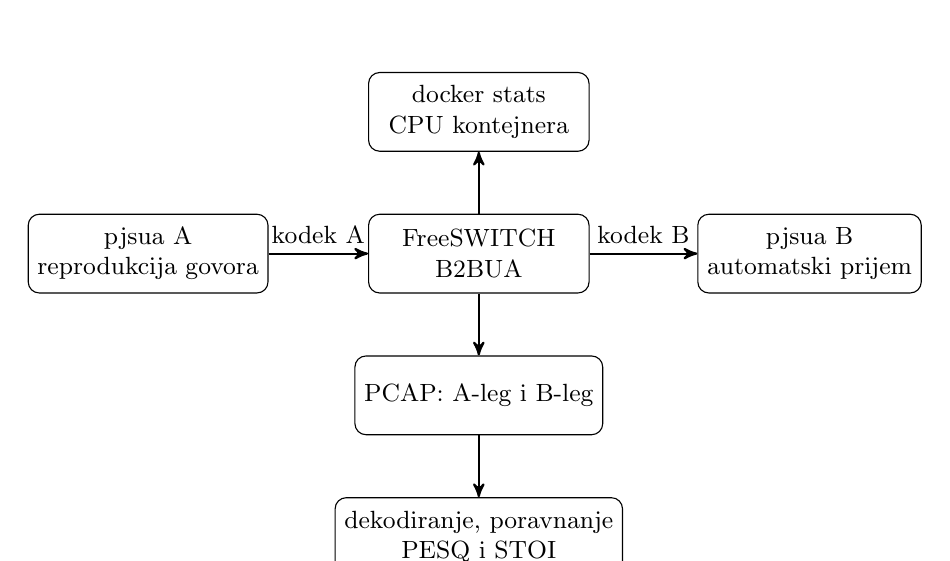
\begin{tikzpicture}[node distance=1.8cm, >=stealth',
    block/.style={rectangle, draw, rounded corners, minimum height=1cm,
                  minimum width=2.8cm, align=center, font=\small},
    arrow/.style={->, thick}]
    \node[block] (a) {pjsua A\\reprodukcija govora};
    \node[block, right of=a, node distance=4.2cm] (fs) {FreeSWITCH\\B2BUA};
    \node[block, right of=fs, node distance=4.2cm] (b) {pjsua B\\automatski prijem};
    \node[block, below of=fs, node distance=1.8cm] (pcap) {PCAP: A-leg i B-leg};
    \node[block, below of=pcap, node distance=1.8cm] (analysis) {dekodiranje, poravnanje\\PESQ i STOI};
    \node[block, above of=fs, node distance=1.8cm] (cpu) {docker stats\\CPU kontejnera};
    \draw[arrow] (a) -- node[above,font=\small]{kodek A} (fs);
    \draw[arrow] (fs) -- node[above,font=\small]{kodek B} (b);
    \draw[arrow] (fs) -- (pcap);
    \draw[arrow] (pcap) -- (analysis);
    \draw[arrow] (fs) -- (cpu);
\end{tikzpicture}
\caption{Eksperimentalni tok i mjesta prikupljanja podataka}
\label{fig:testbed-flow}
\end{figure}

\begin{table}[htbp]
\centering
\caption{Programske komponente konačnog eksperimentalnog okruženja}
\label{tab:software}
\begin{tabular}{|l|l|l|}
\hline
\textbf{Komponenta} & \textbf{Verzija} & \textbf{Uloga} \\
\hline
FreeSWITCH & 1.10.12 & B2BUA i transkodiranje \\
pjsua/PJSIP & 2.14 & krajnji SIP uređaji \\
Docker & 28.1.1 & izolacija FreeSWITCH-a \\
tshark/dumpcap & 3.6.2 & snimanje i čitanje RTP paketa \\
FFmpeg & 4.4.2 & dekodiranje formata kodeka \\
Python & 3.10.12 & automatizacija i analiza \\
\hline
\end{tabular}
\end{table}

Mjerenja su izvršena na računaru s procesorom Intel Core i5-1135G7, četiri fizičke jezgre i osam logičkih procesora, pod operativnim sistemom Ubuntu 22.04 s jezgrom Linux 6.8.0. Budući da kontejner nije imao zadano procesorsko ograničenje, CPU postoci služe za relativno poređenje na ovom računaru.

\section{Testna matrica i ulazni signal}

Ispitano je pet kodeka: PCMU i PCMA na 8 kHz, G.722 na 16 kHz, GSM na 8 kHz i Opus na 48 kHz. Puna usmjerena matrica od $5\times5$ mogućnosti sadrži pet kontrolnih konfiguracija bez transkodiranja i dvadeset konfiguracija s transkodiranjem. Svaka konfiguracija ponovljena je deset puta, pa skup sadrži ukupno \BrojPoziva{} uspješnih poziva.

Svi konačni pozivi izvršeni su sekvencijalno kako se procesorsko opterećenje i mrežni zapis različitih konfiguracija ne bi preklapali. Paketi su slani u okvirima od 20 ms. FreeSWITCH je za Opus u SDP ponudi imao konstantni režim do 30 kbit/s, maksimalnu frekvenciju reprodukcije 48 kHz i parametar \texttt{useinbandfec=0}, dok je pjsua u odgovoru oglasio \texttt{useinbandfec=1}. Kako gubitak paketa nije uveden, razlika FEC postavki nije aktivirana u posmatranim pozivima. Analizirani govorni signal je monofon.

Korišten je monofoni sintetizirani govorni uzorak trajanja 20 sekundi. Generisan je programom eSpeak NG, glasom \texttt{en-us} i brzinom 145 riječi u minuti, iz pet fonetski raznovrsnih engleskih rečenica: ``The birch canoe slid on the smooth planks. Glue the sheet to the dark blue background. These days a chicken leg is a rare dish. Rice is often served in round bowls. The juice of lemons makes fine punch.'' Iz izvornog zapisa izvedene su verzije na 48, 16 i 8 kHz programom FFmpeg. Aktivni RTP tok trajao je približno 12 sekundi; nakon vremenskog poravnanja i uklanjanja rubnih intervala analizirano je približno 10,7 do 10,9 sekundi. Upotreba samo jednog sintetiziranog glasa ograničava generalizaciju na druge govornike, jezike i akustične uslove.

\section{PCAP postupak}

Na lokalnom interfejsu pokreće se dumpcap, odnosno tshark ako dumpcap nije dostupan. Iz snimljenog saobraćaja izdvajaju se dugi RTP tokovi i identificiraju prema smjeru, portovima, SSRC oznaci i vrsti korisnog sadržaja. Za analizu su potrebna dva toka:

\begin{itemize}
    \item kanal A (A-leg), koji krajnji uređaj A šalje prema FreeSWITCH-u i koji predstavlja ulaz u server;
    \item kanal B (B-leg), koji FreeSWITCH šalje prema krajnjem uređaju B i koji predstavlja izlaz iz servera.
\end{itemize}

Za svaki RTP paket izdvajaju se redni broj, vremenska oznaka i korisni sadržaj. PCMU, PCMA, G.722 i GSM mogu se predati FFmpegu kao sirovi tokovi odgovarajućih kodeka. Opus RTP nema kontejnerska zaglavlja, pa skripta gradi Ogg Opus wrapper s poljima OpusHead i OpusTags, vremenskim položajima i kontrolnim sumama. Nakon dekodiranja se za oba kraka, prema razlikama RTP vremenskih oznaka, kao nulti PCM okviri vraćaju intervali koji bi nestali prostim spajanjem korisnih sadržaja. Ovaj postupak pretpostavlja okvire trajanja 20 ms i lokalni prijenos bez promjene redoslijeda paketa.

Dekodirani signali kraka A i kraka B prvo se rekonstruiraju prema RTP vremenskim oznakama, a zatim svode na 16 kHz. Vremenski pomak određuje se unakrsnom korelacijom, odnosno traženjem položaja na kojem se signali najbolje podudaraju. Pretražuje se raspon od $\pm500$ ms. Nakon poravnanja zadržava se zajednički dio signala i uklanja po 0,5 s s njegovog početka i kraja. Nad poravnanim signalima računaju se PESQ MOS-LQO i STOI. Dobijeni pomak služi za tehničku kontrolu poravnanja; ne tumači se kao precizno krajnje mrežno kašnjenje.

Ispravnost izbora tokova dodatno je provjerena na kontrolnim konfiguracijama. Korisni sadržaji izlaznog RTP toka pojavljuju se istim redoslijedom u ulaznom toku, što potvrđuje da se porede odgovarajući kanali. U svih 250 poziva redni brojevi bili su neprekinuti, a promjene vremenskih oznaka odgovarale su cijelom broju okvira. Na kraku A nije bilo vremenskih praznina, dok su na kraku B vraćena dva do osam okvira, prosječno 4,308 okvira po pozivu. Kontrola Opus$\rightarrow$Opus ipak je dala niži PESQ rezultat od ostalih kontrola. Zbog toga se Opus rezultati tumače u odnosu na njegovu vlastitu kontrolu, a ne kao apsolutna ocjena tog kodeka.

\section{Dopunska end-to-end obrada}

Dopunska analiza ne pokreće nove pozive. Za svih 250 postojećih PCAP zapisa ponovo se identifikuje i dekodira B-leg, dok se kao referenca učitava ona verzija izvornog WAV-a koja je stvarno reproducirana za kodek A: 8 kHz za PCMU, PCMA i GSM, 16 kHz za G.722 te 48 kHz za Opus. Povezivanje reference s konfiguracijom zato ne zavisi od naknadne procjene kodeka nego od unaprijed definisane testne matrice.

Prosto spajanje RTP korisnih sadržaja može vremenski sabiti rekonstruisani signal. Ako razlika uzastopnih vremenskih oznaka predstavlja više od jednog očekivanog koraka, između dekodiranih okvira umeće se odgovarajući broj nultih PCM okvira. Time se čuva RTP vremenska linija:

\begin{equation}
N_{\mathrm{prazno}}=\max\!\left(0,\operatorname{round}\!\left(\frac{t_{i+1}-t_i}{f_{RTP}T_p}\right)-1\right).
\end{equation}

Umetanje nultih PCM okvira znači da se nedostajući interval predstavlja tišinom. To je konzervativan pristup jer stvarni uređaj može koristiti algoritam za prikrivanje gubitka paketa, a njegov rezultat nije sadržan u PCAP zapisu. U posmatranom skupu nisu pronađene praznine u RTP rednim brojevima; vraćeni intervali određeni su promjenama vremenske oznake između susjednih paketa. Kod Opusa Ogg dekoder dosljedno preskače četiri početna okvira, što se uzima u obzir prije rekonstrukcije vremenske linije.

Original i rekonstruisani B-leg prvo se svode na 16 kHz. Unakrsna korelacija nad središnjih 80\% zapisa traži pomak unutar $\pm500$ ms, nakon čega se odstranjuje po 0,5 s s oba ruba zajedničkog intervala. Dobijeni par koristi se za WB PESQ i STOI. Za izvore na 8 kHz dodatno se formira par na 8 kHz i računa NB PESQ; za širokopojasne izvore izvorni PESQ režim jednak je WB postupku na 16 kHz. Referentne tačke primarne i dopunske analize prikazane su na Slici~\ref{fig:reference-boundaries}.

Za dopunsku spektralnu provjeru nad svih 250 poravnatih parova Welchovom metodom procijenjena je spektralna snaga~\cite{welch1967}. Udio energije u opsegu 3,4--7 kHz računat je u odnosu na ukupnu energiju između 80 Hz i 7,9 kHz. Za vizuelni prikaz konfiguracije Opus$\rightarrow$GSM odabrana je iteracija čiji je end-to-end PESQ najbliži prosjeku te konfiguracije, čime se izbjegava izbor ekstremnog primjera. Ova analiza je deskriptivna i ne zamjenjuje PESQ ili STOI.

\begin{figure}[htbp]
\centering
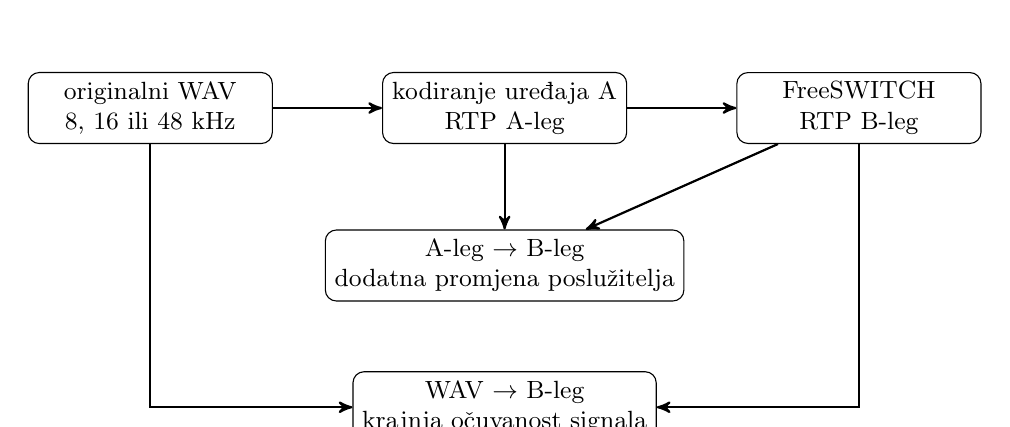
\begin{tikzpicture}[node distance=1.7cm, >=stealth',
    block/.style={rectangle, draw, rounded corners, minimum height=0.9cm,
                  minimum width=3.1cm, align=center, font=\small},
    arrow/.style={->, thick}]
    \node[block] (wav) {originalni WAV\\8, 16 ili 48 kHz};
    \node[block, right of=wav, node distance=4.5cm] (aleg) {kodiranje uređaja A\\RTP A-leg};
    \node[block, right of=aleg, node distance=4.5cm] (bleg) {FreeSWITCH\\RTP B-leg};
    \node[block, below of=aleg, node distance=2.0cm] (server) {A-leg $\rightarrow$ B-leg\\dodatna promjena poslužitelja};
    \node[block, below of=server, node distance=1.8cm] (e2e) {WAV $\rightarrow$ B-leg\\krajnja očuvanost signala};
    \draw[arrow] (wav) -- (aleg);
    \draw[arrow] (aleg) -- (bleg);
    \draw[arrow] (aleg) -- (server);
    \draw[arrow] (bleg) -- (server);
    \draw[arrow] (wav) |- (e2e);
    \draw[arrow] (bleg) |- (e2e);
\end{tikzpicture}
\caption{Referentne tačke primarne i dopunske analize}
\label{fig:reference-boundaries}
\end{figure}

Validacija je provedena prije grupne analize. Svih 250 analiza završilo je uspješno, svaka od 25 konfiguracija ima deset rezultata, a kontrolne sume potvrđuju 250 različitih PCAP datoteka. Nisu pronađene praznine u rednim brojevima ni necjelobrojni skokovi vremenske oznake. Pomaci su ostali unutar zadanog prozora, a poravnati interval trajao je između 10,80 i 10,98 s. Time se provjerava tehnička konzistentnost obrade, ali se ne uklanja ograničenje rekonstrukcije Opus toka u Ogg wrapper.

\section{Mjerenje procesorskog opterećenja}

Tokom svakog probnog poziva naredba \texttt{docker stats} periodično bilježi ukupnu potrošnju procesora FreeSWITCH kontejnera. Prosjek obuhvata aktivni poziv i kratke pripremne intervale te uključuje osnovno opterećenje kontejnera. Zbog trajanja pojedinačnog očitanja prikupljeno je približno osam uzoraka po pozivu. Mjera je pogodna za relativno poređenje konfiguracija izvršenih na istom računaru, ali nije dovoljna za procjenu najvećeg broja istovremenih produkcijskih poziva.

\section{Obrada i statistička analiza}

Za svaku konfiguraciju računati su aritmetička sredina i standardna devijacija deset ponavljanja. Dodatna degradacija konfiguracije $A\rightarrow B$ definisana je u odnosu na kontrolu istog izvornog kodeka:
\begin{equation}
\Delta_{A\rightarrow B}=\overline{PESQ}_{A\rightarrow A}-\overline{PESQ}_{A\rightarrow B}.
\end{equation}
Time svaki transkodirani rezultat ima odgovarajuću referentnu vrijednost, a kodeci su jednako zastupljeni. Rezultati se prvenstveno opisuju prosjecima i razlikama jer matrica sadrži sve usmjerene parove odabranih kodeka. Dodatno je provjereno razlikuje li se prosječna degradacija od nule. Za tu provjeru korišten je dvostrani jednouzorački $t$-test nad 20 konfiguracija. Prikazani su i 95-postotni interval pouzdanosti te korigirana Hedgesova mjera veličine efekta. Izračuni su izvedeni bibliotekama NumPy i SciPy~\cite{scipy}; deset tehničkih ponavljanja ne tretira se kao deset nezavisnih govornika.

\section{Ponovljivost}

Konačni skup sadrži po jedan JSON zapis, PCAP zapis i historiju CPU opterećenja za svaki od \BrojPoziva{} poziva. Sažetak u CSV i JSON formatu generiše se iz tih zapisa, a tabele u ovom dokumentu iz sažetka. Docker slika je vezana za tačan digest, a neposredne Python zavisnosti za tačne verzije. Time se smanjuje mogućnost da nova instalacija neprimjetno promijeni eksperimentalno okruženje~\cite{docker-handbook,pjsip}.

\chapter{Rezultati i analiza}
\label{ch:rezultati}

Analizirana je puna matrica od \BrojKonfiguracija{} konfiguracija kodeka sa po deset uspješnih ponavljanja, ukupno \BrojPoziva{} poziva. Sve vrijednosti u ovom poglavlju automatski su izvedene iz pojedinačnih JSON zapisa. PESQ MOS-LQO poredi signal ulaznog kraka A i izlaznog kraka B te zato predstavlja dodatnu promjenu kroz server, a ne apsolutni kvalitet u odnosu na izvorni govor.

\section{Kontrolne konfiguracije}

% Automatski generisano; ne uređivati ručno.
\begin{table}[htbp]
\centering
\caption{Rezultati prijenosa bez transkodiranja}
\label{tab:passthrough-details}
\begin{tabular}{|l|c|c|c|c|}
\hline
\textbf{Test} & \textbf{Kodek} & \textbf{PESQ MOS-LQO} & \textbf{STOI} & \textbf{CPU (\%)} \\
\hline
T001 & PCMU & 4,412 $\pm$ 0,213 & 0,998 & 2,04 \\
T002 & PCMA & 4,311 $\pm$ 0,215 & 0,997 & 1,99 \\
T003 & G.722 & 4,401 $\pm$ 0,139 & 0,998 & 1,96 \\
T004 & Opus & 3,792 $\pm$ 0,205 & 0,992 & 1,97 \\
T005 & GSM & 4,296 $\pm$ 0,181 & 0,996 & 2,09 \\
\hline
\textbf{Prosjek} & & \textbf{4,242} & \textbf{0,996} & \textbf{2,01} \\
\hline
\end{tabular}
\end{table}


PCMU, PCMA i G.722 daju rezultate blizu gornjeg dijela skale. Opus je niži iako nema promjene kodeka. Provjerom RTP korisnih sadržaja utvrđeno je da se izlazni okviri kontrolnih konfiguracija pojavljuju istim redoslijedom u ulaznom toku, ali početak, kraj i manji broj unutrašnjih okvira nisu jednaki. Na rezultat zato mogu utjecati raspoređivanje medija u serveru, rekonstrukcija Ogg Opus toka i vremensko poravnanje. Opus kontrola koristi se kao njegova vlastita osnovna vrijednost, rezultat nije dokaz slabijeg apsolutnog kvaliteta kodeka.

\section{Scenariji s transkodiranjem}

Prosječni PESQ MOS-LQO konfiguracija s transkodiranjem iznosi \TranscodePESQ. Za svaku konfiguraciju dodatna degradacija $\Delta$ računata je u odnosu na kontrolu njenog izvornog kodeka. Prosjek dvadeset vrijednosti iznosi \RazlikaPESQ{} MOS-LQO boda, a nijedna transkodirana konfiguracija nije nadmašila odgovarajuću kontrolu.

% Automatski generisano; ne uređivati ručno.
\begin{table}[htbp]
\centering
\caption{Scenariji s najmanjom i najvećom dodatnom degradacijom}
\label{tab:transcode-extremes}
\small
\begin{tabular}{|l|c|c|c|}
\hline
\textbf{Kombinacija} & \textbf{PESQ MOS-LQO} & \textbf{$\Delta$PESQ} & \textbf{CPU (\%)} \\
\hline
GSM $\rightarrow$ PCMU & 4,279 $\pm$ 0,186 & 0,017 & 2,59 \\
PCMA $\rightarrow$ PCMU & 4,191 $\pm$ 0,121 & 0,120 & 1,38 \\
GSM $\rightarrow$ PCMA & 4,172 $\pm$ 0,254 & 0,124 & 1,33 \\
PCMU $\rightarrow$ PCMA & 4,202 $\pm$ 0,159 & 0,210 & 2,02 \\
\hline
G.722 $\rightarrow$ GSM & 2,246 $\pm$ 0,039 & 2,155 & 2,63 \\
PCMU $\rightarrow$ GSM & 2,492 $\pm$ 0,093 & 1,920 & 2,34 \\
PCMA $\rightarrow$ GSM & 2,548 $\pm$ 0,057 & 1,763 & 2,18 \\
Opus $\rightarrow$ GSM & 2,298 $\pm$ 0,158 & 1,494 & 3,26 \\
\hline
\end{tabular}
\end{table}


Prosjeci prema odredišnom kodeku iznose \ProsjekPremaOpusu{} za Opus, \ProsjekPremaPCMU{} za PCMU, \ProsjekPremaPCMA{} za PCMA, \ProsjekPremaGSevenTwoTwo{} za G.722 i \ProsjekPremaGSMu{} za GSM. Budući da puna matrica za svaki odredišni kodek sadrži po četiri različita izvora, ti prosjeci imaju jednaku težinu. Kodiranje u Opus uglavnom bolje čuva ulazni signal, ali zahtijeva više procesorskih resursa, dok smjerovi prema GSM-u daju najveću dodatnu degradaciju. Vrijednosti svih konfiguracija prikazane su na Slici~\ref{fig:pesq-bars}, puna matrica prema izvornom i odredišnom kodeku na Slici~\ref{fig:heatmap}, a dodatna degradacija na Slici~\ref{fig:pesq-degradation}.

\begin{figure}[htbp]
\centering
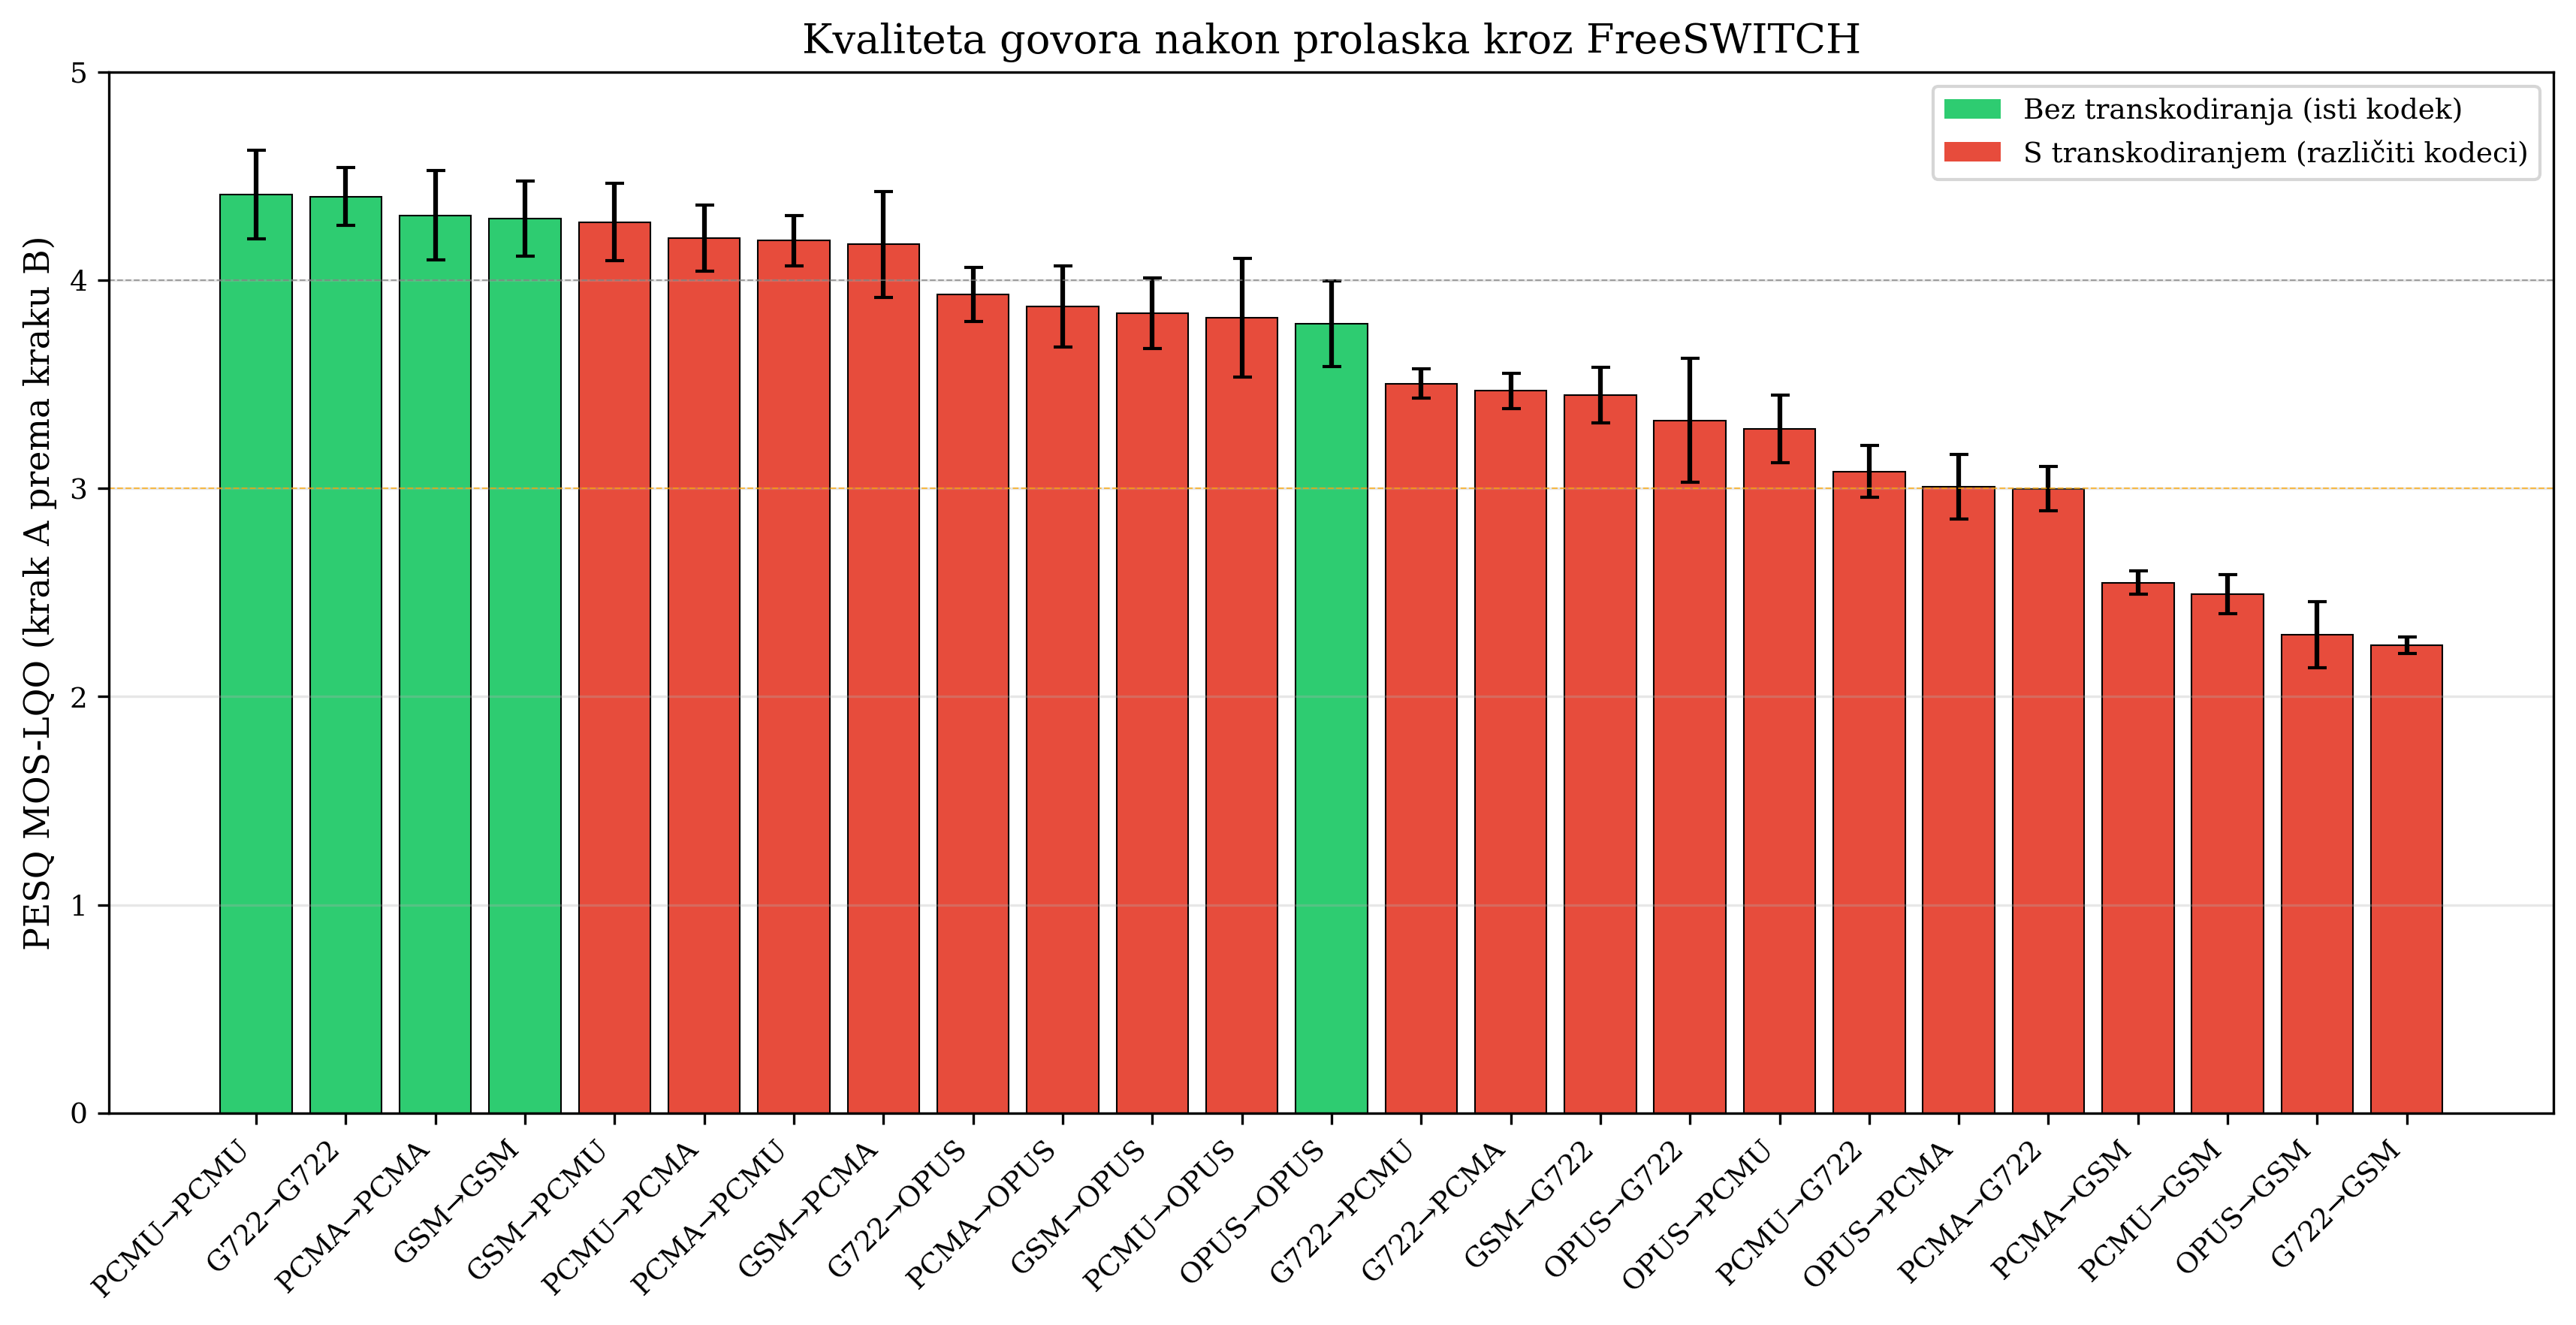
\includegraphics[width=0.95\textwidth]{pesq_mos_bars.png}
\caption{PESQ MOS-LQO za sve kombinacije; greške prikazuju uzoračku standardnu devijaciju deset ponavljanja}
\label{fig:pesq-bars}
\end{figure}

\begin{figure}[htbp]
\centering
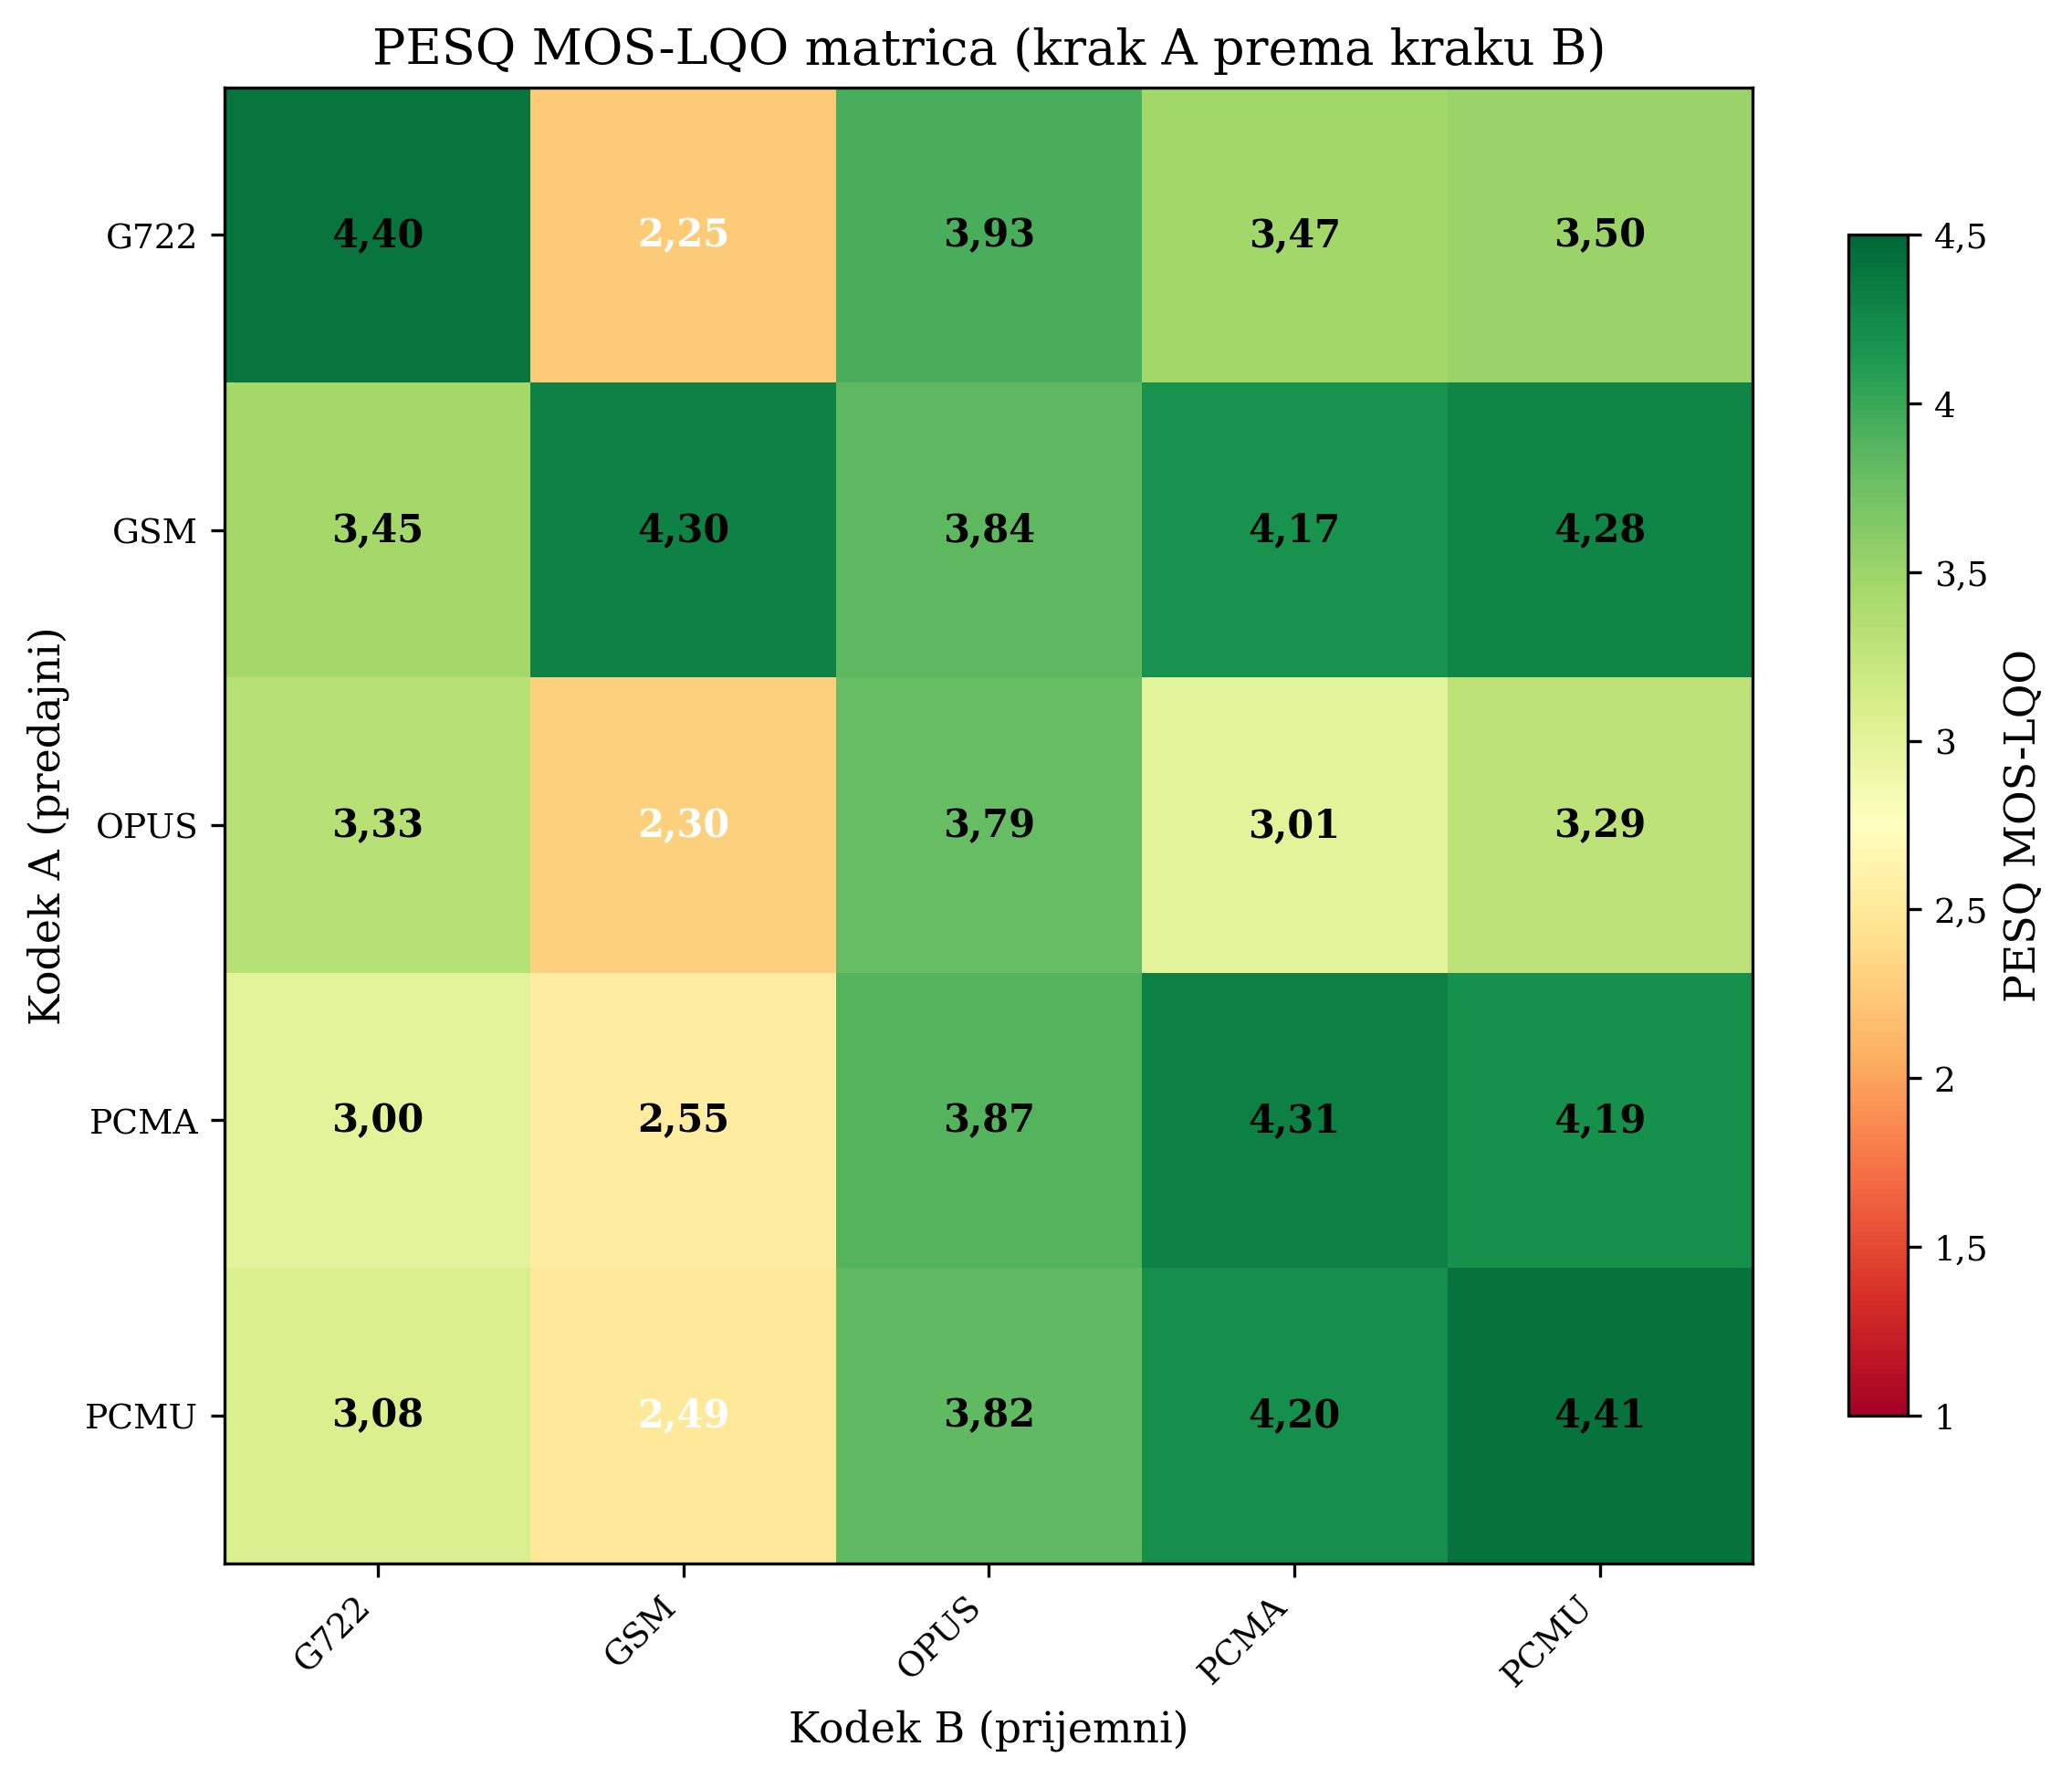
\includegraphics[width=0.85\textwidth]{codec_heatmap.png}
\caption{Puna matrica PESQ MOS-LQO rezultata}
\label{fig:heatmap}
\end{figure}

\begin{figure}[htbp]
\centering
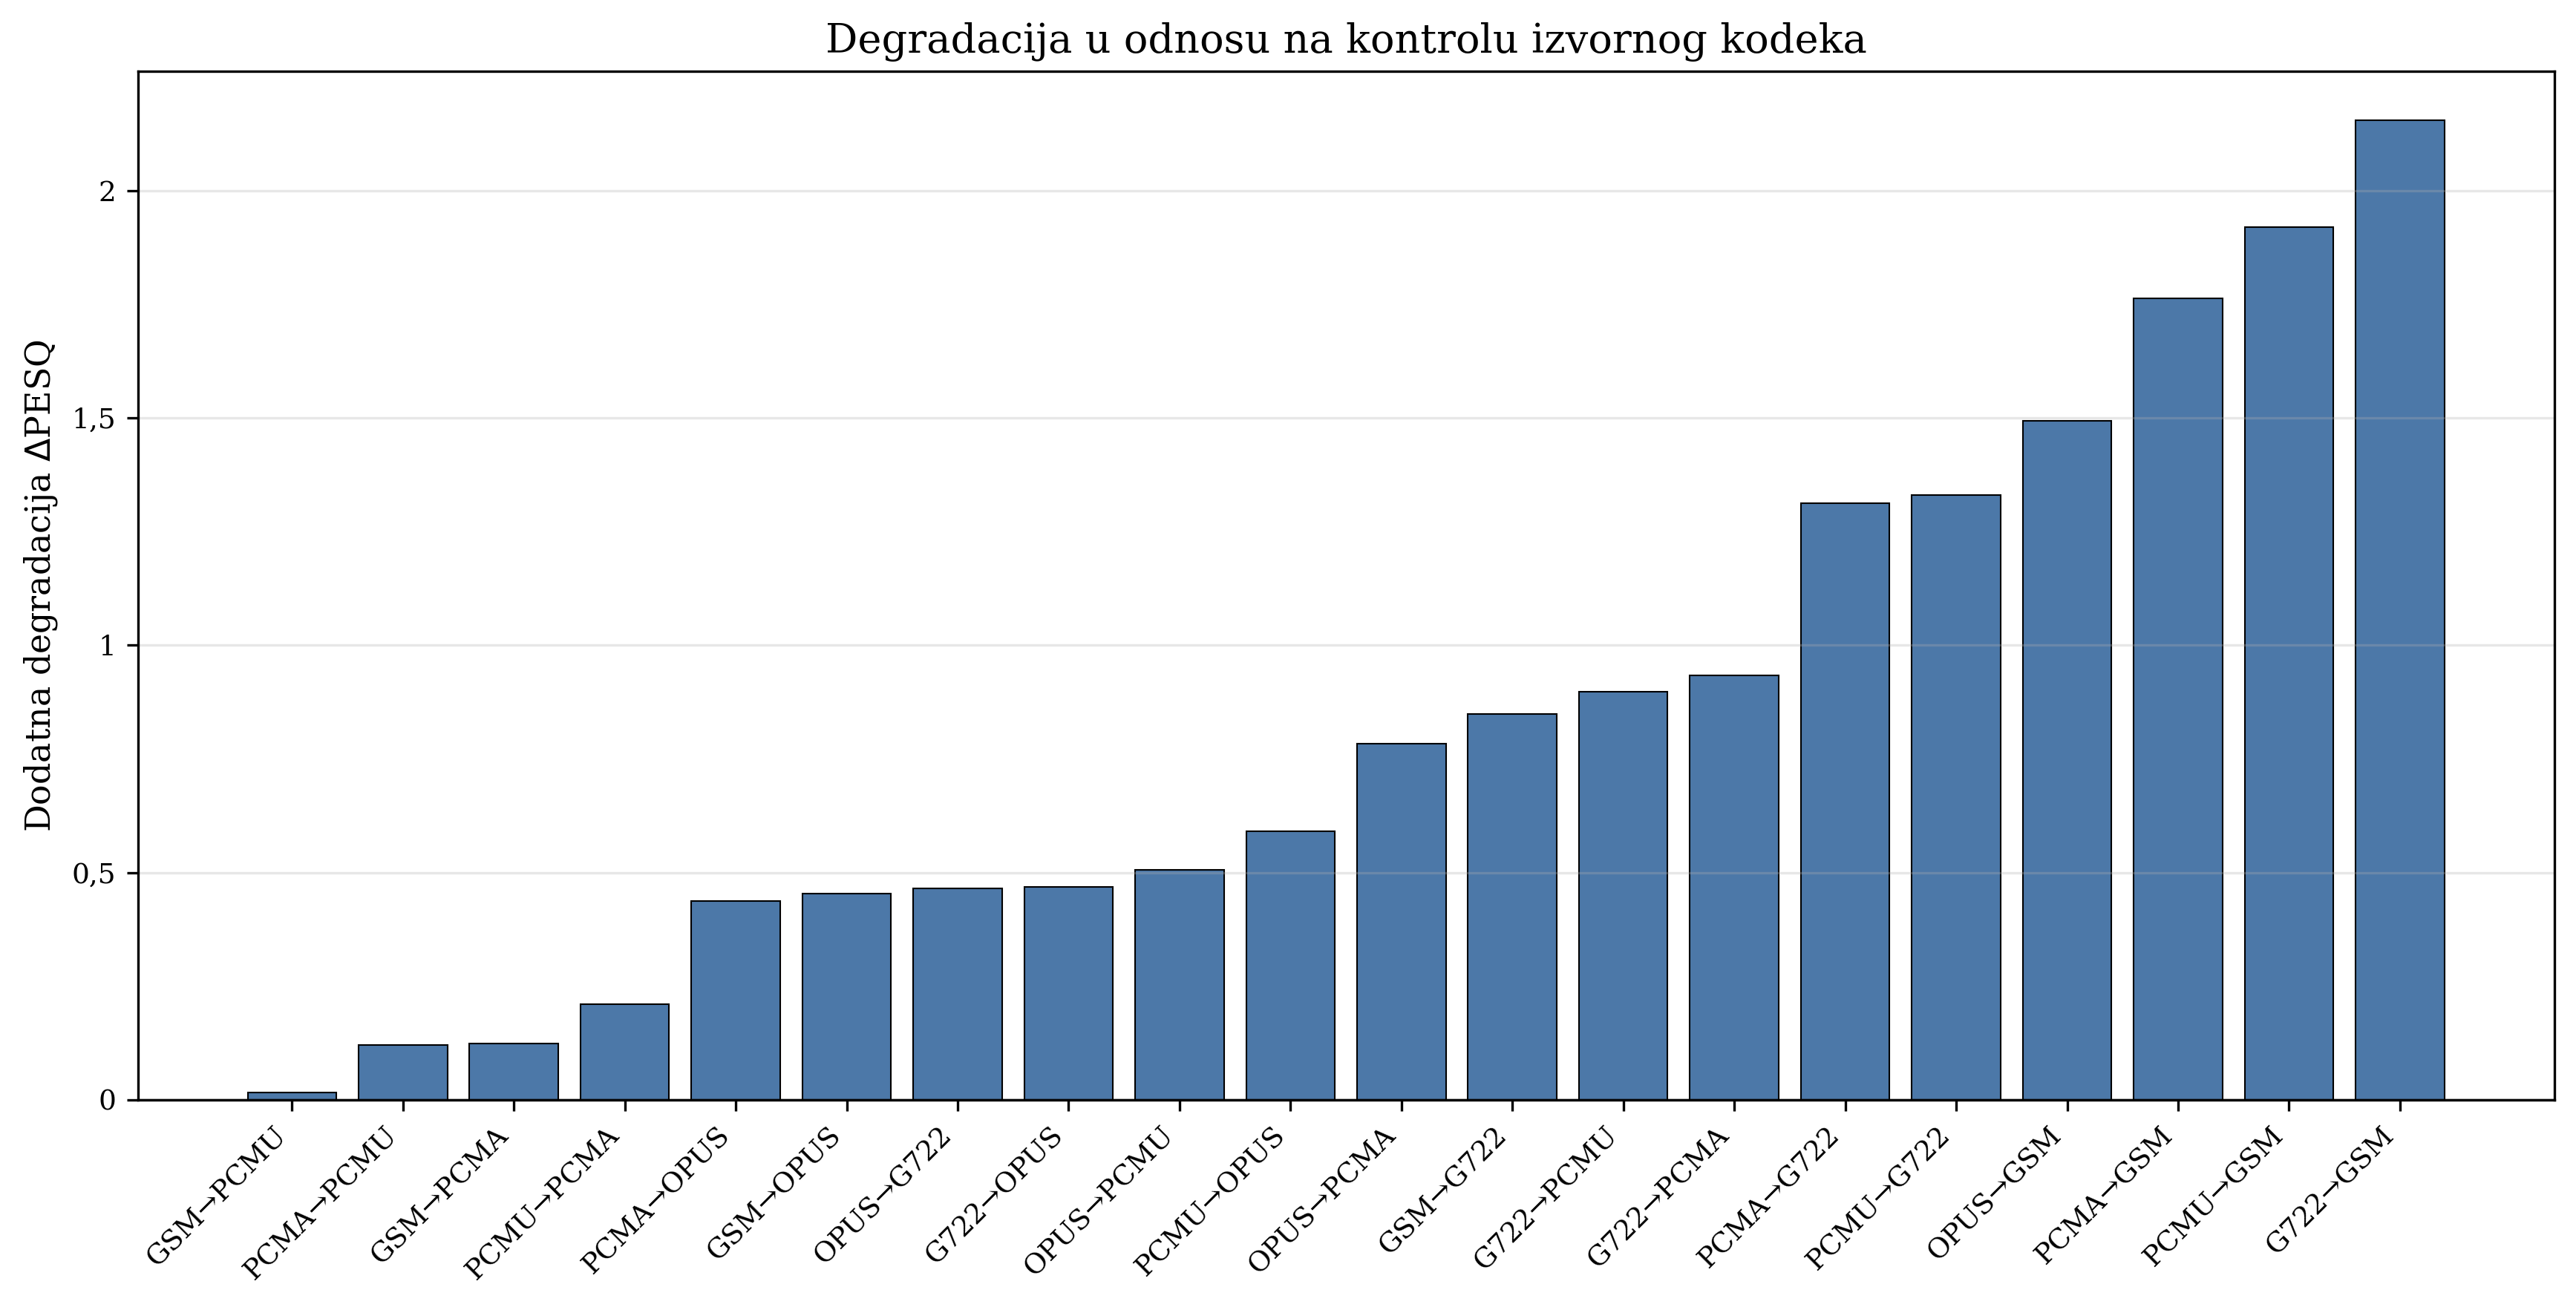
\includegraphics[width=0.95\textwidth]{pesq_degradation.png}
\caption{Dodatna degradacija u odnosu na kontrolu istog izvornog kodeka}
\label{fig:pesq-degradation}
\end{figure}

\FloatBarrier
\section{Utjecaj smjera konverzije}

Rezultati su usmjereni: $A\rightarrow B$ i $B\rightarrow A$ obuhvataju različit odredišni koder i, kod kodeka različitog opsega, različitu promjenu frekvencije uzorkovanja. Tabela~\ref{tab:directional-asymmetry} zato neposredno uspoređuje svih deset neuređenih parova.

% Automatski generisano; ne uređivati ručno.
\begin{table}[htbp]
\centering
\caption{Razlika rezultata između suprotnih smjerova transkodiranja}
\label{tab:directional-asymmetry}
\small
\begin{tabular}{|l|c|c|c|}
\hline
\textbf{Par kodeka} & \textbf{prvi$\rightarrow$drugi} & \textbf{drugi$\rightarrow$prvi} & \textbf{Apsolutna razlika} \\
\hline
PCMU/PCMA & 4,202 & 4,191 & 0,011 \\
PCMU/G.722 & 3,081 & 3,504 & 0,423 \\
PCMU/Opus & 3,821 & 3,286 & 0,535 \\
PCMU/GSM & 2,492 & 4,279 & 1,787 \\
PCMA/G.722 & 2,999 & 3,468 & 0,469 \\
PCMA/Opus & 3,874 & 3,009 & 0,865 \\
PCMA/GSM & 2,548 & 4,172 & 1,624 \\
G.722/Opus & 3,932 & 3,327 & 0,605 \\
G.722/GSM & 2,246 & 3,448 & 1,202 \\
Opus/GSM & 2,298 & 3,842 & 1,544 \\
\hline
\end{tabular}
\end{table}


Razlike između suprotnih smjerova potvrđuju da se rezultat jednog smjera ne smije preslikati na drugi. To je praktično važno pri definisanju prioriteta kodeka jer ista dva krajnja formata mogu dati različitu dodatnu degradaciju zavisno od toga koji se koristi na izlaznom kraku.

\section{Eksplorativna statistička provjera}

Primarni nalaz je deskriptivan jer matrica sadrži sve usmjerene parove pet odabranih kodeka. Kao dopunska provjera, dvadeset konfiguracijskih vrijednosti $\Delta_{A\rightarrow B}$ uspoređeno je s nulom. Dvostrani test daje $t=\DeltaT$ uz \DeltaDF{} stepeni slobode i $p=\DeltaP$. Prosječna dodatna degradacija iznosi \RazlikaPESQ{} MOS-LQO boda. Njen 95-postotni interval pouzdanosti kreće se od \RazlikaCIDonja{} do \RazlikaCIGornja{}, a korigirana Hedgesova mjera iznosi $g=\HedgesG$. Test opisuje razlike među odabranim konfiguracijama. Deset tehničkih ponavljanja ne predstavlja deset različitih govornika, pa se rezultat ne može proširiti na sve moguće kodeke i govornike.

\section{STOI i procesorsko opterećenje}

Prosječni STOI kontrolnih konfiguracija iznosi približno 0,996, dok kod konfiguracija s transkodiranjem ostaje visok. STOI se ovdje računa u odnosu na krak A, a promjene frekvencije uzorkovanja i različite osnovne vrijednosti kodeka utječu na grupni prosjek. Zato se koristi kao pomoćna provjera očuvanja razumljivosti, bez tvrdnje da transkodiranje može poboljšati izvorni govor.

Prosječno opterećenje FreeSWITCH kontejnera iznosi \PassthroughCPU{} bez transkodiranja i \TranscodeCPU{} s transkodiranjem, odnosno približno \OmjerCPU{} puta više. Najveće vrijednosti imaju konfiguracije koje kodiraju u Opus. Pošto mjerenje obuhvata cijeli kontejner, osnovno opterećenje i dio pripremnog intervala, rezultat je relativna usporedba na ispitnom računaru, a ne univerzalna cijena jednog poziva. Vrijednosti po konfiguraciji prikazane su na Slici~\ref{fig:cpu-bars}.

\begin{figure}[htbp]
\centering
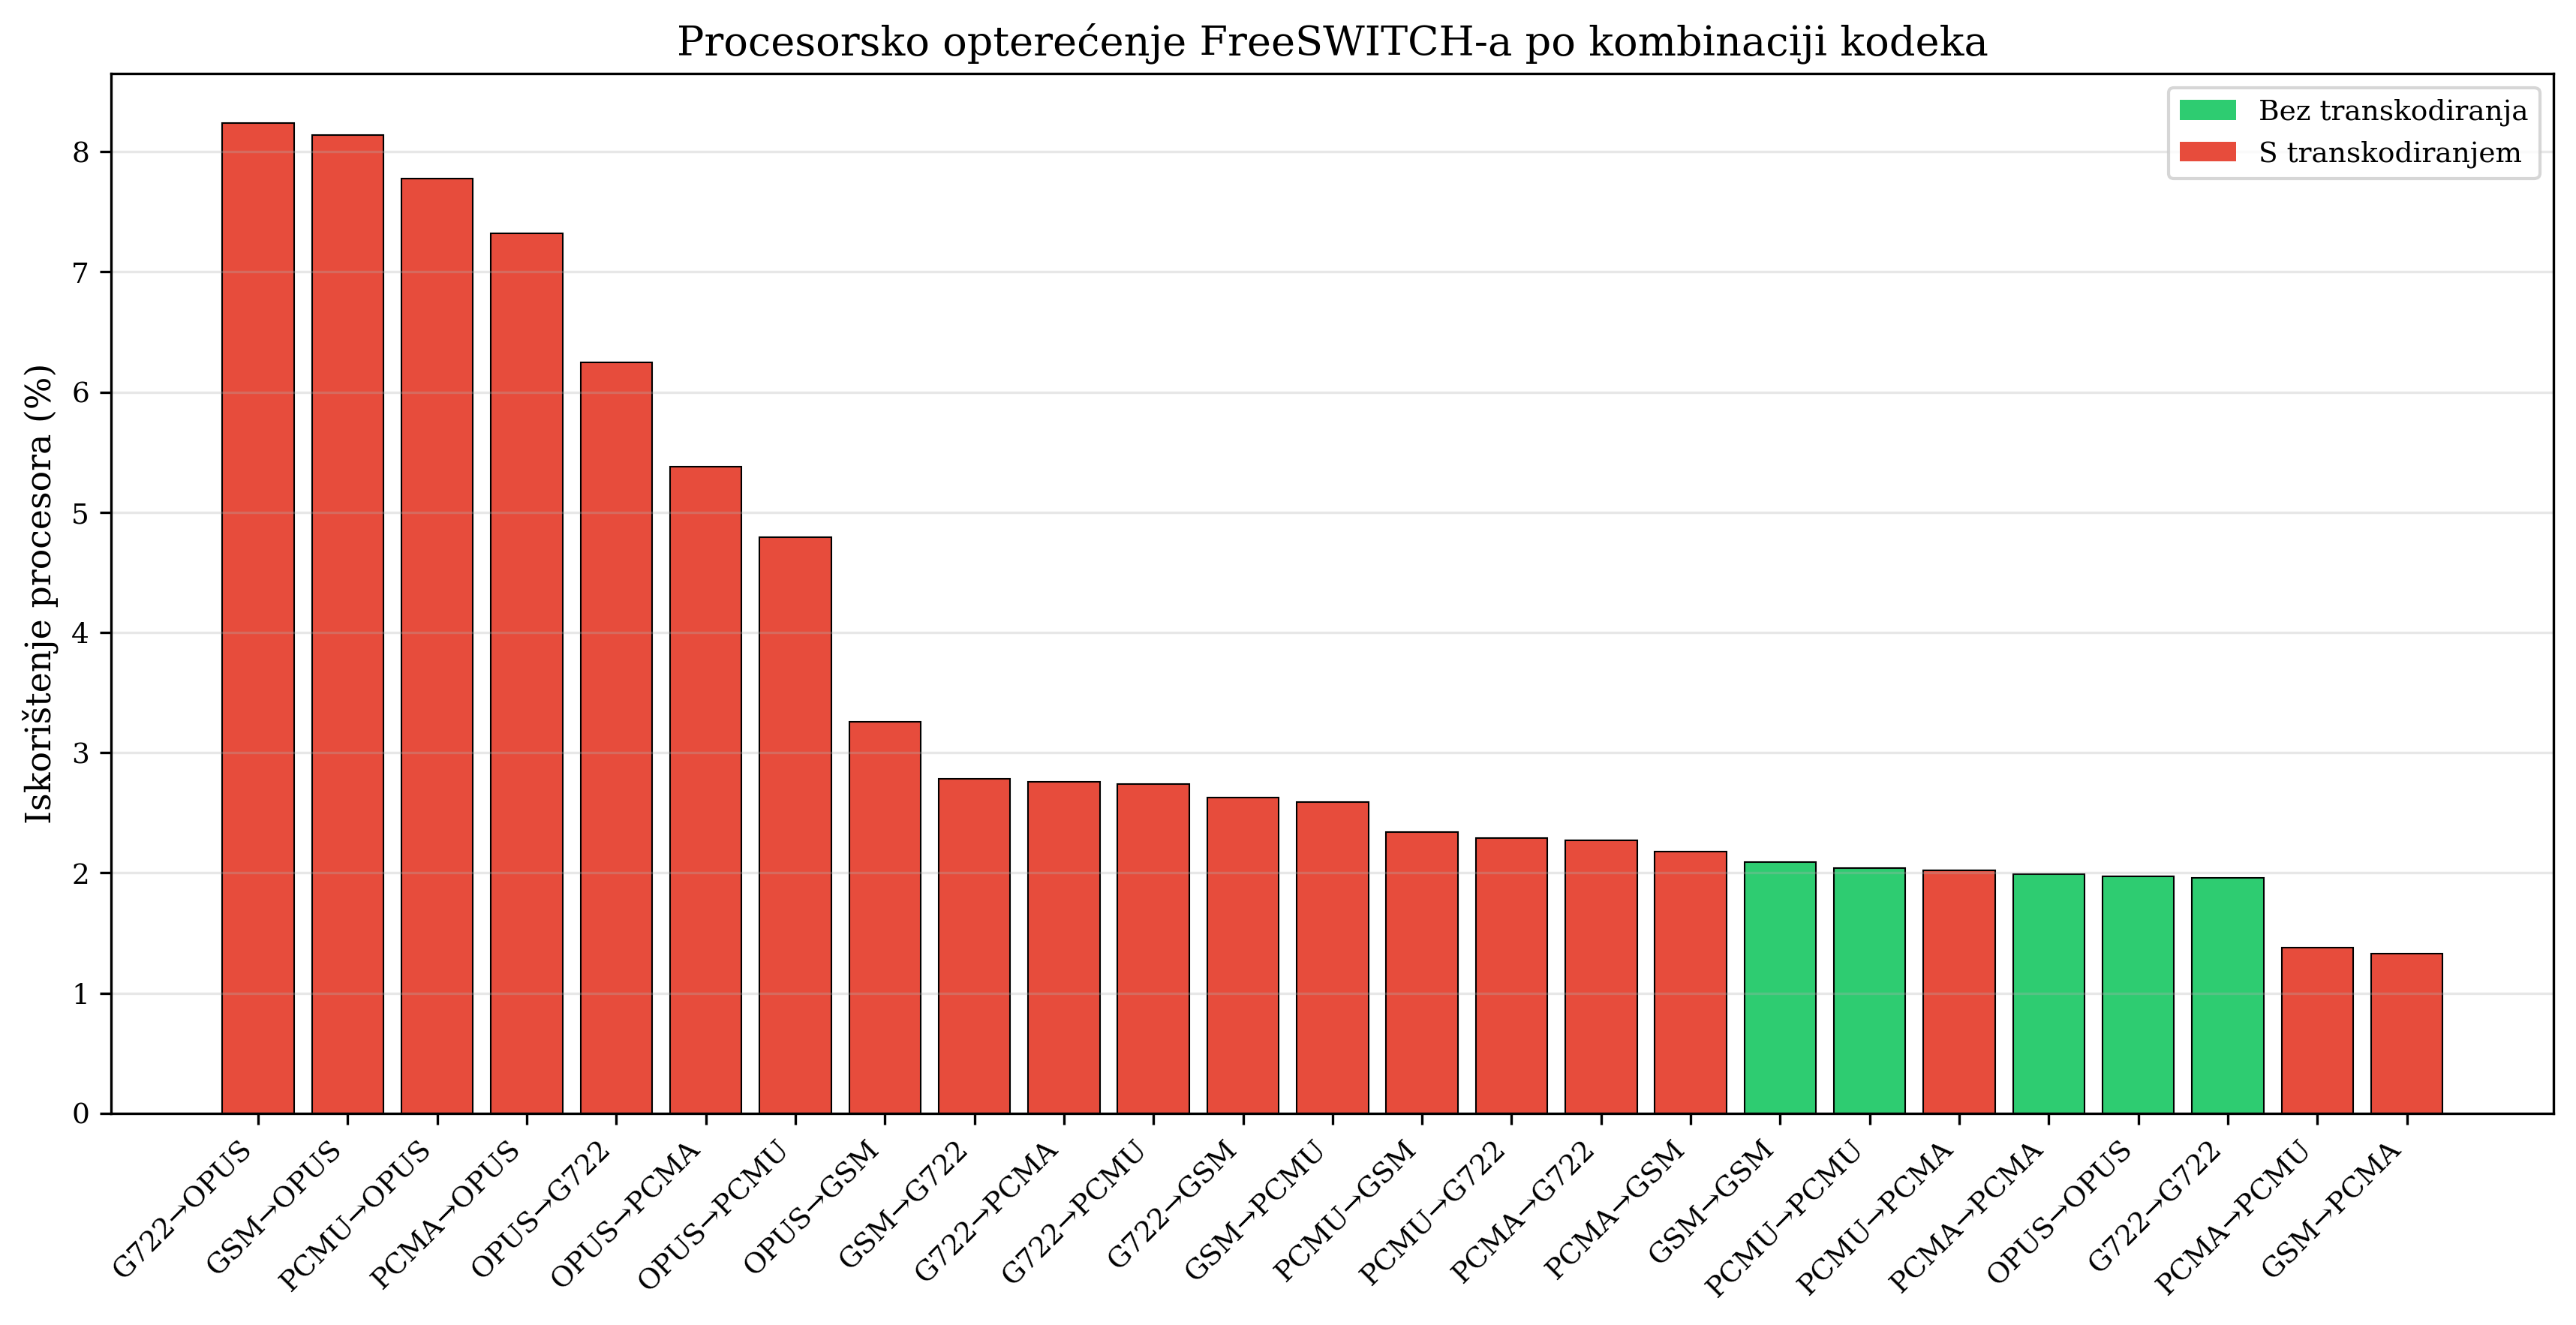
\includegraphics[width=0.95\textwidth]{cpu_usage_bars.png}
\caption{Prosječna potrošnja procesora FreeSWITCH kontejnera po konfiguraciji}
\label{fig:cpu-bars}
\end{figure}

\FloatBarrier
\section{Dopunska end-to-end analiza}
\label{sec:e2e-results}

Primarna analiza pokazuje koliko se B-leg razlikuje od signala koji je FreeSWITCH primio na A-legu. Dopunska analiza koristi originalni reproducirani WAV kao referencu i zato uključuje početno kodiranje kodekom A, obradu na serveru i završno kodiranje kodekom B. Za istih 250 poziva prosječni WB PESQ na 16 kHz iznosi 3,170 za pet kontrola bez transkodiranja i 2,608 za dvadeset transkodiranih konfiguracija. Odgovarajući prosjeci STOI su 0,983 i 0,932.

Na nivou pojedinačnih poziva WB PESQ je u rasponu 1,750--3,944, a STOI u rasponu 0,817--0,996. Raspon nije sam po sebi rang-lista kodeka: svaka konfiguracija uključuje ograničenje izvornog kodeka A, a vrijednost zavisi i od odredišnog kodera. Zbog toga se transkodirana putanja poredi s end-to-end kontrolom istog izvora. Prosjek tako definisane dodatne degradacije iznosi 0,563 PESQ boda.

% Izvor: results/end_to_end_original_vs_bleg_20260828/summary_by_configuration.csv
\begin{table}[htbp]
\centering
\caption{End-to-end rezultat prema izvornom kodeku na kraku A}
\label{tab:e2e-by-source}
\small
\begin{tabular}{|l|c|c|c|c|}
\hline
\textbf{Izvor A} & \textbf{Kontrola} & \textbf{Prosjek ostalih} & \textbf{Prosječni $\Delta$} & \textbf{STOI ostalih} \\
\hline
PCMU  & 3,688 & 2,982 & 0,706 & 0,9625 \\
PCMA  & 3,708 & 3,013 & 0,695 & 0,9535 \\
G.722 & 2,868 & 2,435 & 0,433 & 0,9685 \\
GSM   & 2,294 & 2,229 & 0,065 & 0,9213 \\
Opus  & 3,294 & 2,381 & 0,913 & 0,8555 \\
\hline
\end{tabular}
\end{table}


Tabela~\ref{tab:e2e-by-source} pokazuje zašto je izbor reference važan. GSM kontrola već ima WB PESQ 2,294 prema originalu. Ostale putanje koje počinju GSM-om prosječno daju 2,229, pa je dodatna razlika samo 0,065. Mali dodatni gubitak ne znači visok apsolutni kvalitet, nego da kasniji koder uglavnom čuva signal koji je već ograničen GSM kodiranjem. Suprotno tome, Opus kontrola iznosi 3,294, a prosjek njegovih transkodiranih izlaza 2,381, jer odredišni uskopojasni kodeci odbacuju dio informacije prisutan na ulazu. Odnosi svih izvornih i odredišnih kodeka prikazani su na Slici~\ref{fig:e2e-heatmap}.

\begin{figure}[htbp]
\centering
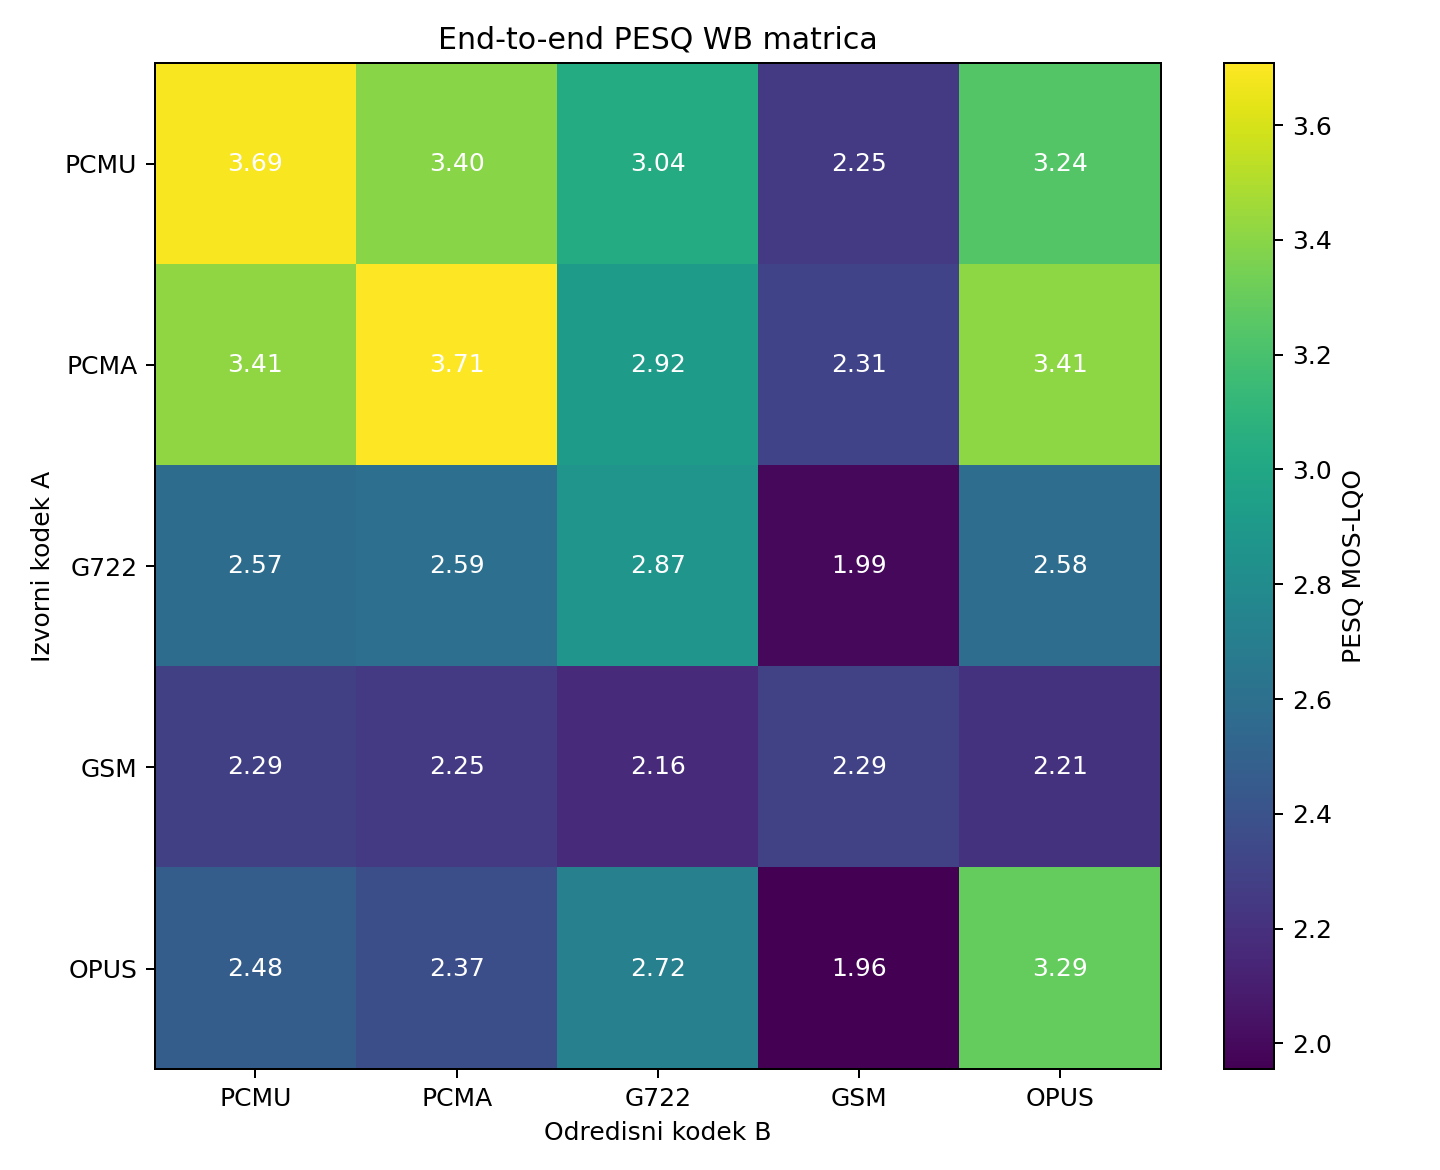
\includegraphics[width=0.82\textwidth]{../results/end_to_end_original_vs_bleg_20260828/charts/pesq_wb_16k_heatmap.png}
\caption{End-to-end WB PESQ matrica: originalni WAV prema izlaznom B-legu}
\label{fig:e2e-heatmap}
\end{figure}

Najviše apsolutne WB PESQ vrijednosti među transkodiranim konfiguracijama imaju sljedeće putanje:

\begin{itemize}
    \item PCMA$\rightarrow$PCMU: 3,414;
    \item PCMA$\rightarrow$Opus: 3,408;
    \item PCMU$\rightarrow$PCMA: 3,396.
\end{itemize}

Njihov izvor nije prethodno prošao kroz snažno kompresijski govorni model, a odredište ne uvodi uskopojasno kodiranje niske brzine poput GSM-a. Najniže vrijednosti imaju Opus$\rightarrow$GSM (1,955) i G.722$\rightarrow$GSM (1,993), gdje se širokopojasni izvor svodi na uskopojasni GSM format.

Spektralna analiza dodatno pokazuje šta se događa u smjeru Opus$\rightarrow$GSM. Posmatrano kroz svih deset ponavljanja, prosječni udio energije u opsegu 3,4--7 kHz smanjen je sa 2,84\% u izvornom signalu na 0,08\% u krajnjem B-legu. Frekvencija ispod koje se nalazi 95\% spektralne energije pomjerena je sa 2763 Hz na 1646 Hz. Na Slici~\ref{fig:opus-gsm-spectrum} prikazana je reprezentativna peta iteracija, čiji je PESQ najbliži prosjeku konfiguracije. Vremenski oblik zadržava osnovnu strukturu govora, dok spektrogram i prosječna raspodjela spektralne snage jasno pokazuju potiskivanje viših frekvencija nakon kodiranja u GSM.

\begin{figure}[htbp]
\centering
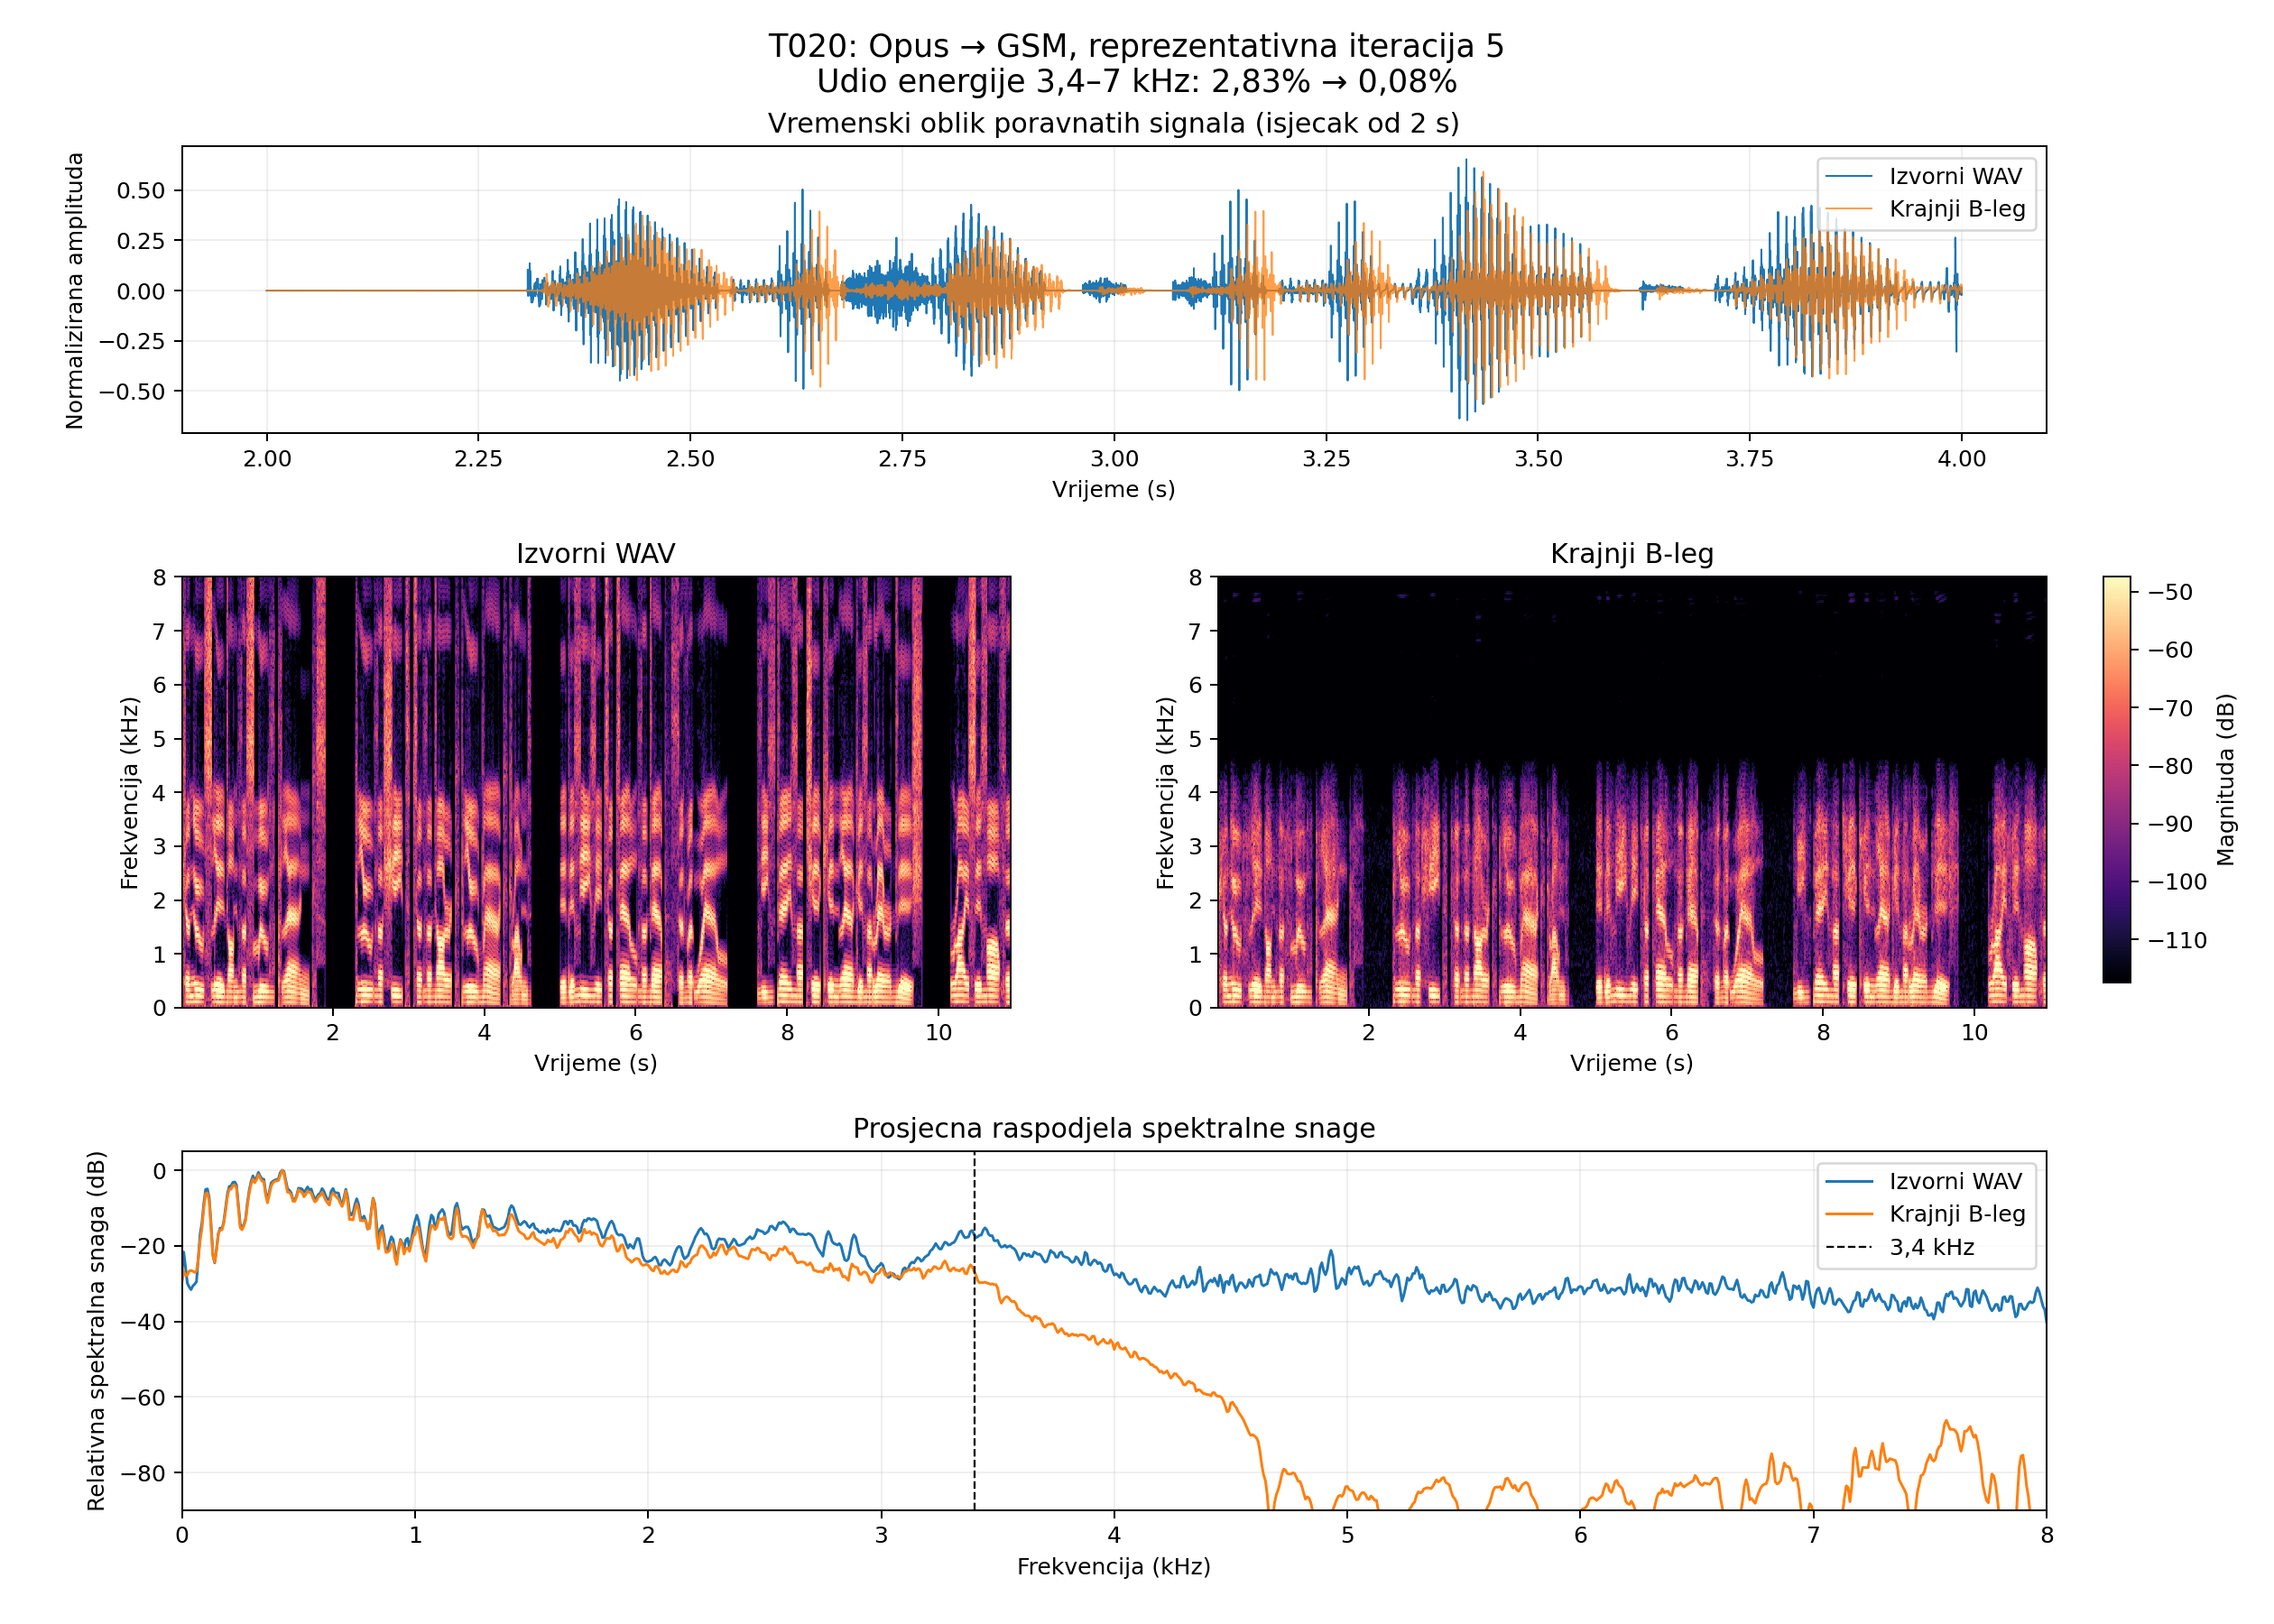
\includegraphics[width=0.98\textwidth]{opus_to_gsm_signal_comparison.png}
\caption{Poređenje izvornog signala i krajnjeg B-lega za konfiguraciju Opus$\rightarrow$GSM}
\label{fig:opus-gsm-spectrum}
\end{figure}

Isti obrazac vidi se u dodatnoj degradaciji prema kontroli izvornog kodeka. Najveće vrijednosti imaju PCMU$\rightarrow$GSM (1,434), PCMA$\rightarrow$GSM (1,398) i Opus$\rightarrow$GSM (1,339). Najmanje su GSM$\rightarrow$PCMU (0,006), GSM$\rightarrow$PCMA (0,039) i GSM$\rightarrow$Opus (0,082). U prvom skupu završni GSM koder odbacuje znatan dio preostale informacije; u drugom skupu odredišni kodek malo mijenja već GSM-ograničeni signal.

Posebno ilustrativna je konfiguracija GSM$\rightarrow$PCMA. A-leg$\rightarrow$B-leg PESQ iznosi 4,172, što pokazuje da je FreeSWITCH vrlo malo promijenio ulazni GSM signal. End-to-end WB PESQ ipak iznosi 2,255 jer je najveći dio razlike prema originalu nastao prije ulaska u poslužitelj. Dodatna end-to-end degradacija u odnosu na GSM kontrolu iznosi samo 0,039 boda. Bez obje referentne tačke rezultat 4,172 mogao bi se pogrešno protumačiti kao visok konačni kvalitet. Poređenje svih konfiguracija prikazano je na Slici~\ref{fig:e2e-bars}.

\begin{figure}[htbp]
\centering
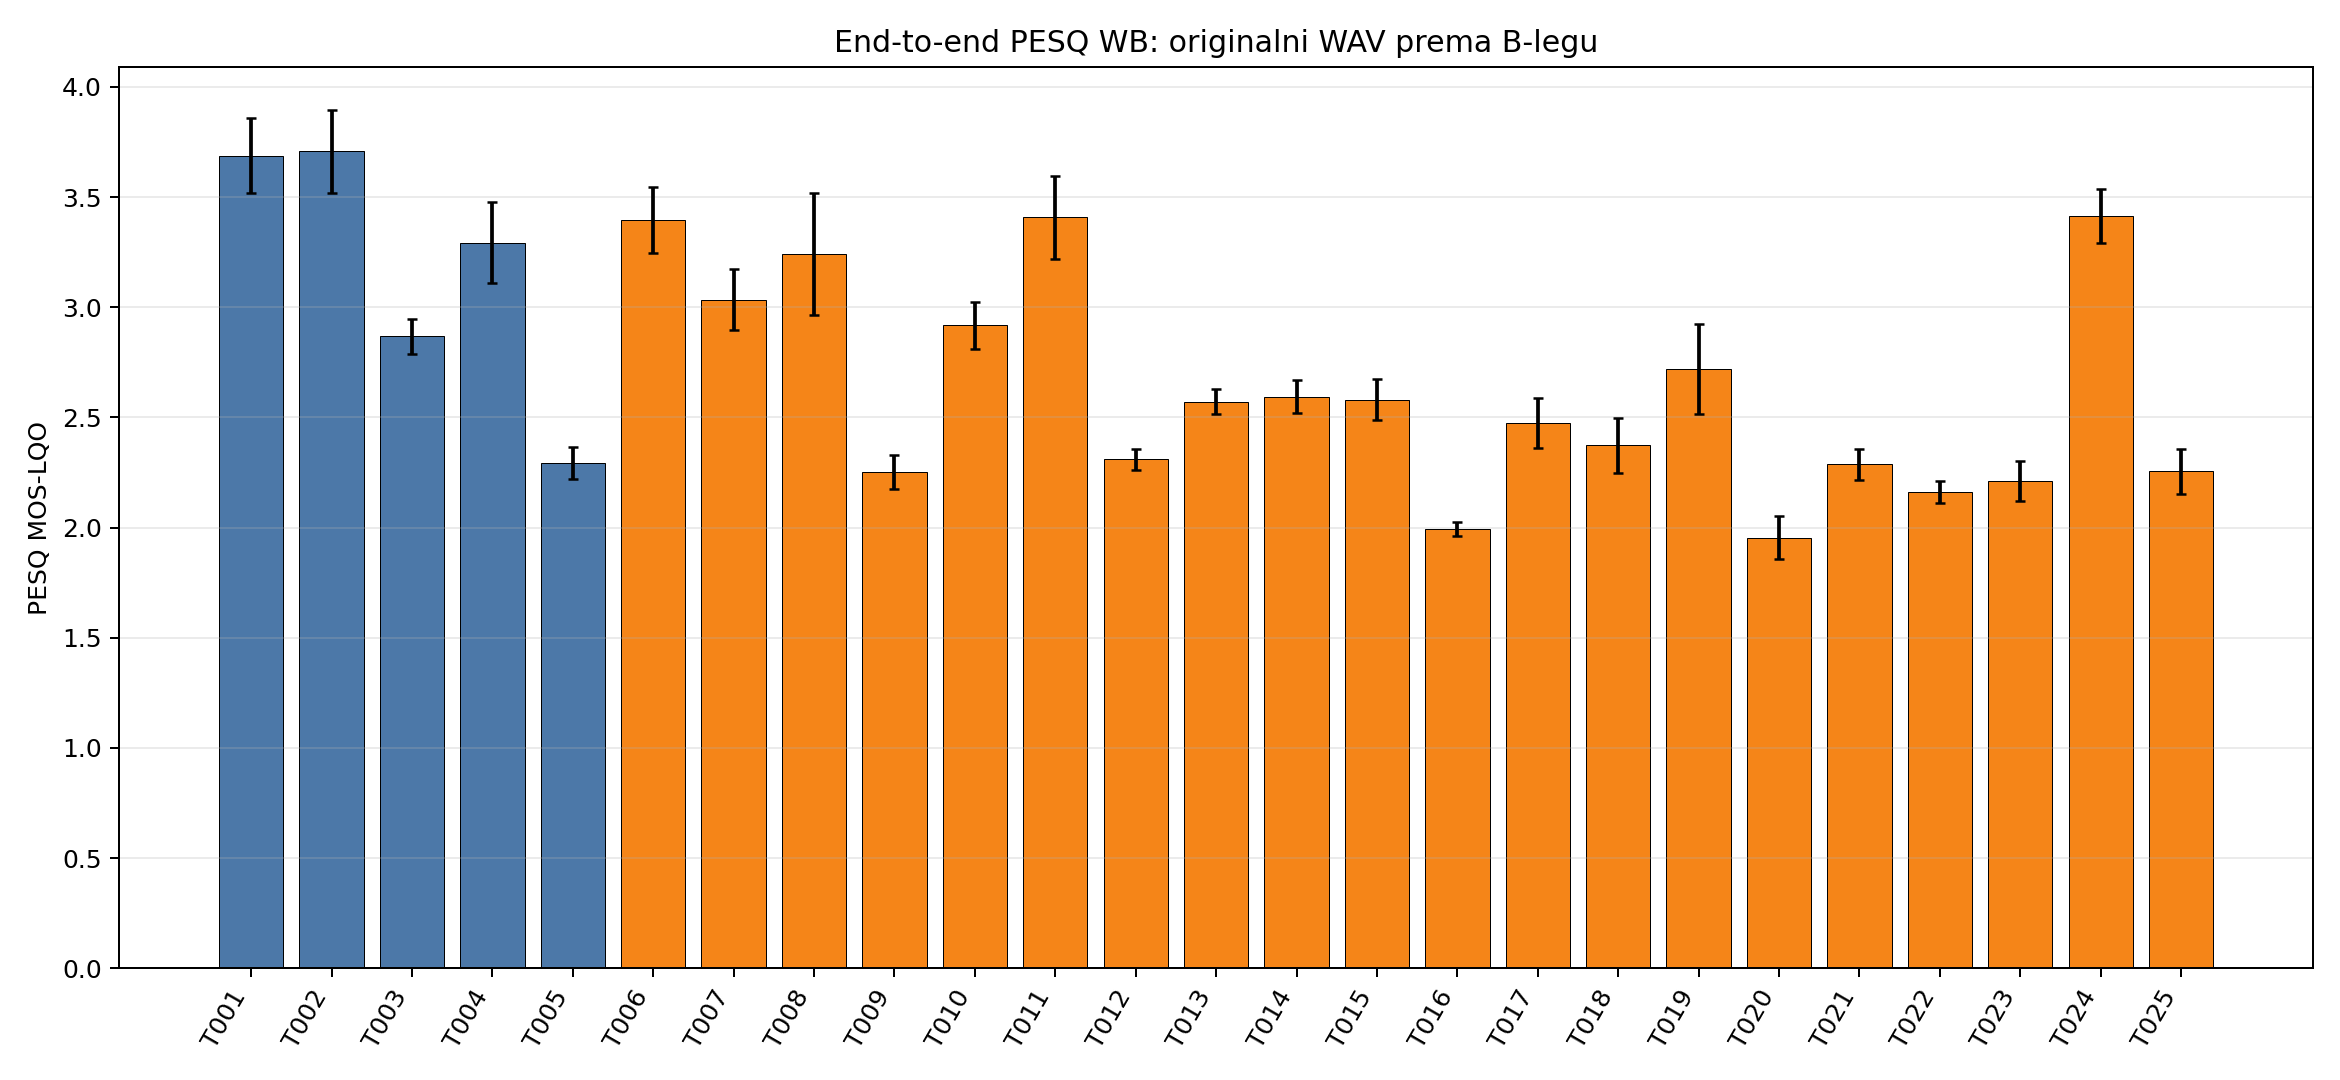
\includegraphics[width=0.95\textwidth]{../results/end_to_end_original_vs_bleg_20260828/charts/pesq_wb_16k_bars.png}
\caption{End-to-end WB PESQ po konfiguraciji; greške prikazuju standardnu devijaciju deset ponavljanja}
\label{fig:e2e-bars}
\end{figure}

Pored zajedničkog WB postupka, izračunat je PESQ u režimu izvornog opsega: NB na 8 kHz za PCMU, PCMA i GSM izvore, a WB na 16 kHz za G.722 i Opus. Taj prikaz je prikladniji za uskopojasne izvore, ali NB i WB vrijednosti ne treba objedinjavati u jednu rang-listu. Zaključci o tome koje putanje dodaju najmanje ili najviše degradacije ostaju kvalitativno usklađeni s fizičkim ograničenjima kodeka.

End-to-end STOI ostaje visok kod većine konfiguracija, što znači da je struktura važna za razumljivost uglavnom očuvana i kada PESQ bilježi perceptivnu degradaciju. Varijabilnost je izraženija u putanjama s Opusom, naročito kada je Opus izvor. Ovaj dio rezultata treba tumačiti uz ograničenje rekonstrukcije RTP Opus okvira u Ogg wrapper. Zbog toga PESQ i STOI predstavljaju dopunske, a ne međusobno zamjenjive pokazatelje.

Tehničke provjere uspješno su završene za svih 250 zapisa. Svaka konfiguracija ima deset rezultata, a svih 250 PCAP zapisa je jedinstveno. RTP vremenske oznake imaju pravilne cjelobrojne skokove. Sva poravnanja ostala su unutar zadanog vremenskog raspona. Time je dopunska analiza dovoljno konzistentna za usporedbu s primarnim nalazima, uz navedena ograničenja reference i Opus rekonstrukcije.

\section{Praktične implikacije}

Rezultati podržavaju korištenje zajedničkog kodeka na oba kraja kada je to moguće. Ako je transkodiranje neizbježno, politiku kodeka treba zasnivati na konkretnom smjeru, prihvatljivoj degradaciji, raspoloživoj propusnosti i procesorskom kapacitetu. U ovom okruženju kodiranje u Opus daje povoljan odnos očuvanja ulaznog signala i propusnosti u primarnoj analizi, ali uz najveće CPU opterećenje. End-to-end rezultati dodatno pokazuju da prelazak u širokopojasni format ne može vratiti sadržaj izgubljen u prethodnom uskopojasnom kodeku. Kodiranje u GSM zato treba ograničiti na slučajeve u kojima kompatibilnost ili ušteda propusnosti opravdavaju izmjerenu degradaciju.

Politika prioriteta u SDP ponudi treba uzeti u obzir oba kanala. Ako krajnji uređaji imaju zajednički prihvatljiv kodek, njegovo zadržavanje uklanja jednu fazu dekodiranja i ponovnog kodiranja. Direktna konverzija PCMU$\leftrightarrow$PCMA u ovom skupu ima relativno malu degradaciju jer ostaje na istoj frekvenciji uzorkovanja i koristi srodne PCM predstavnike. Ipak, rezultat nije potpuno identičan prolazu zbog različitih kvantizacijskih nivoa. Putanje prema GSM-u pokazuju suprotan slučaj: smanjena propusnost plaća se najvećim gubitkom kvaliteta, posebno kada je ulaz širokopojasan.

Za nadzor produkcijskog sistema korisno je odvojeno prikazivati dvije vrste pokazatelja. A-leg$\rightarrow$B-leg mjera pomaže otkriti neuobičajenu degradaciju u medijskom serveru, dok mjera original$\rightarrow$B-leg pokazuje šta na kraju ostaje od polaznog signala. Bez prve se uzrok lošeg rezultata teško lokalizuje, a bez druge dobar rezultat nakon već degradiranog izvora može izgledati bolje nego što ga korisnik čuje. Praktični nadzor zato treba povezati kodeke oba kraka, mrežne pokazatelje i procesorsko opterećenje sa jasno označenom referentnom tačkom kvaliteta.

CPU rezultati ne određuju kapacitet poslužitelja, ali pokazuju koje putanje treba posebno testirati pri dimenzioniranju i skaliranju. Veći broj istovremenih Opus kodera može postati ograničenje prije mrežne propusnosti, dok G.711 troši više mrežnog kapaciteta uz jednostavniju obradu. Konačna politika zato nije samo rangiranje PESQ vrijednosti: ona je izbor kompromisa između očuvanosti govora, dostupne propusnosti, broja istovremenih poziva i skupa kodeka koje podržavaju povezane mreže.

\chapter{Zaključak}
\label{ch:zakljucak}

U radu je razvijeno i primijenjeno okruženje za mjerenje promjene govornog signala pri transkodiranju u FreeSWITCH-u. Glavna vrijednost pristupa jeste izdvajanje ulaznog kanala A i izlaznog kanala B neposredno iz RTP paketa, čime se posmatra obrada na medijskom serveru bez oslanjanja na njegove interne PCM snimke. Dopunsko poređenje originalnog WAV-a i B-lega pokazuje konačnu očuvanost signala, a koristi iste snimljene pozive bez pokretanja novih testova.

\section{Odgovori na istraživačka pitanja}

Za punu matricu pet kodeka prosječni PESQ MOS-LQO iznosi \PassthroughPESQ{} bez transkodiranja i \TranscodePESQ{} s transkodiranjem. Kada se svaka konfiguracija usporedi sa kontrolom istog izvornog kodeka, prosječna dodatna degradacija iznosi \RazlikaPESQ{} boda. Nalaz je potvrđen eksplorativnom analizom konfiguracijskih razlika, ali ne znači da svaki smjer gubi isti iznos.

Smjer i odredišni kodek imaju velik utjecaj. Kodiranje u Opus uglavnom dobro čuva signal kanala A, dok kodiranje u GSM dodaje najveću degradaciju. Usporedba svih deset parova pokazuje da suprotni smjerovi nisu zamjenjivi, zbog različitog odredišnog kodera i promjene frekvencije uzorkovanja.

Prosječno opterećenje kontejnera približno je \OmjerCPU{} puta veće u grupi s transkodiranjem. Najviše vrijednosti zabilježene su pri kodiranju u Opus. Taj nalaz predstavlja relativnu razliku na ispitnom računaru i nije dovoljan za neposredno dimenzioniranje produkcijskog sistema.

End-to-end analiza potvrđuje da se mala dodatna degradacija ne smije izjednačiti s visokim konačnim kvalitetom. Prosječni WB PESQ iznosi 3,170 za kontrole i 2,608 za transkodirane konfiguracije, uz prosječnu dodatnu degradaciju od 0,563 boda prema kontroli istog izvora. Putanja GSM$\rightarrow$PCMA to jasno pokazuje: A-leg$\rightarrow$B-leg rezultat je 4,172, a rezultat prema originalnom WAV-u 2,255. FreeSWITCH u toj putanji dodaje samo 0,039 boda degradacije, ali ne može nadoknaditi informaciju koju je početni GSM koder već odbacio. Spektralna analiza smjera Opus$\rightarrow$GSM dodatno potvrđuje gubitak viših frekvencija: udio energije u opsegu 3,4--7 kHz smanjen je sa 2,84\% na 0,08\%.

\section{Ograničenja zaključaka}

Mjerenje između kanala A i kanala B izoluje doprinos servera, dok mjerenje od originalnog WAV-a obuhvata cijeli posmatrani kodečki lanac. Nijedno samo po sebi nije potpuna procjena korisničkog iskustva u glasovnom pozivu. Zajednički WB postupak na 16 kHz može utjecati na uskopojasne konfiguracije, pa dopunska analiza prikazuje i PESQ u izvornom NB ili WB režimu. Posebno ponašanje konfiguracija s Opusom pokazuje da na rezultat mogu utjecati rekonstrukcija RTP toka, Ogg wrapper i vremensko poravnanje.

Korišten je jedan sintetizirani glas, bez namjerno uvedenog gubitka paketa i kašnjenja. Eksperiment je proveden na jednom računaru, a CPU mjerenje obuhvata cijeli kontejner, osnovno opterećenje i dio pripremnog intervala. Deset ponavljanja po konfiguraciji procjenjuje tehničku ponovljivost, ali ne zamjenjuje raznolik skup govornika ni subjektivni MOS test prema ITU-T P.800.

\section{Preporuke i budući rad}

U upravljanim VoIP mrežama treba dati prednost zajedničkom kodeku na oba kanala. Kada je transkodiranje potrebno, politike treba zasnivati na konkretnom smjeru, a ne samo na nazivima dva kodeka. Za promet prema Opusu treba planirati veće procesorske resurse, dok GSM kao odredišni kodek treba koristiti kada kompatibilnost ili ušteda propusnosti opravdavaju izmjerenu degradaciju.

Buduća provjera treba koristiti više stvarnih govornika oba spola i ujednačen skup rečenica na jeziku ciljnih korisnika. Potrebno je dodatno provjeriti rekonstrukciju Opus RTP toka. CPU treba mjeriti samo tokom stabilnog aktivnog dijela poziva i nakon oduzimanja osnovnog opterećenja. Ako su dostupne odgovarajuća licenca i referentna implementacija, rezultate treba potvrditi metrikom POLQA. Zaseban eksperiment može kontrolisano uvesti gubitak paketa i kolebanje kašnjenja, porediti različite mehanizme prikrivanja gubitka te uključiti subjektivno slušno ispitivanje.

Zaključno, implementirani sistem daje ponovljiv način poređenja svih usmjerenih kombinacija odabranih kodeka na nivou poslužitelja i cijelog kodečkog lanca. Najvažniji nalaz nije jedna univerzalna vrijednost degradacije, nego činjenica da učinak transkodiranja zavisi od smjera, odredišnog kodeka, prethodno izgubljenog sadržaja, procesorskog troška i izbora referentne tačke.

%%%%%%%%%%%%%%%%%%%%% PRILOZI %%%%%%%%%%%%%%%%%%%%%%%%%%%%%%%%%%%%
\begin{appendices}
% Prilozi se nalaze u odvojenim datotekama.
%Prilog 1
\chapter{Dodatni podaci}
\label{app:rezultati}

\section{Kompletna tabela rezultata}

U Tabeli~\ref{tab:complete-results} prikazani su rezultati automatski generisani iz datoteke \path{results/summary/results_summary.csv}. Takav postupak osigurava da su vrijednosti u prilogu usklađene s konačnim rezultatima analize.

% Automatski generisano; ne uređivati ručno.
% Izvor: results/summary/results_summary.csv
\begin{table}[htbp]
\centering
\caption{Rezultati za sve ispitane kombinacije (prosjek $\pm$ standardna devijacija, 10 ponavljanja)}
\label{tab:complete-results}
\scriptsize
\begin{tabular}{|l|l|l|c|c|c|}
\hline
\textbf{Test} & \textbf{Kodek A} & \textbf{Kodek B} & \textbf{PESQ MOS-LQO} & \textbf{STOI} & \textbf{CPU (\%)} \\
\hline
T001 & PCMU & PCMU & 4,412 $\pm$ 0,213 & 0,998 & 2,04 \\
T002 & PCMA & PCMA & 4,311 $\pm$ 0,215 & 0,997 & 1,99 \\
T003 & G.722 & G.722 & 4,401 $\pm$ 0,139 & 0,998 & 1,96 \\
T004 & Opus & Opus & 3,792 $\pm$ 0,205 & 0,992 & 1,97 \\
T005 & GSM & GSM & 4,296 $\pm$ 0,181 & 0,996 & 2,09 \\
\hline
T006 & PCMU & PCMA & 4,202 $\pm$ 0,159 & 0,994 & 2,02 \\
T007 & PCMU & G.722 & 3,081 $\pm$ 0,125 & 0,994 & 2,29 \\
T008 & PCMU & Opus & 3,821 $\pm$ 0,285 & 0,926 & 7,78 \\
T009 & PCMU & GSM & 2,492 $\pm$ 0,093 & 0,946 & 2,34 \\
T010 & PCMA & G.722 & 2,999 $\pm$ 0,105 & 0,992 & 2,27 \\
T011 & PCMA & Opus & 3,874 $\pm$ 0,196 & 0,889 & 7,32 \\
T012 & PCMA & GSM & 2,548 $\pm$ 0,057 & 0,949 & 2,18 \\
T013 & G.722 & PCMU & 3,504 $\pm$ 0,071 & 0,993 & 2,74 \\
T014 & G.722 & PCMA & 3,468 $\pm$ 0,086 & 0,992 & 2,76 \\
T015 & G.722 & Opus & 3,932 $\pm$ 0,129 & 0,951 & 8,24 \\
T016 & G.722 & GSM & 2,246 $\pm$ 0,039 & 0,950 & 2,63 \\
T017 & Opus & PCMU & 3,286 $\pm$ 0,163 & 0,869 & 4,79 \\
T018 & Opus & PCMA & 3,009 $\pm$ 0,155 & 0,865 & 5,38 \\
T019 & Opus & G.722 & 3,327 $\pm$ 0,297 & 0,856 & 6,25 \\
T020 & Opus & GSM & 2,298 $\pm$ 0,158 & 0,845 & 3,26 \\
T021 & GSM & PCMU & 4,279 $\pm$ 0,186 & 0,995 & 2,59 \\
T022 & GSM & G.722 & 3,448 $\pm$ 0,134 & 0,992 & 2,78 \\
T023 & GSM & Opus & 3,842 $\pm$ 0,169 & 0,863 & 8,14 \\
T024 & PCMA & PCMU & 4,191 $\pm$ 0,121 & 0,994 & 1,38 \\
T025 & GSM & PCMA & 4,172 $\pm$ 0,254 & 0,994 & 1,33 \\
\hline
\end{tabular}
\end{table}


\section{Sljedivost podataka}

Konačni skup obuhvata \BrojPoziva{} JSON zapisa, \BrojPoziva{} PCAP zapisa i \BrojPoziva{} dnevnika procesorskog opterećenja. Za svaku konfiguraciju dostupno je deset uspješnih ponavljanja. Prva 23 skupa mjerenja prikupljena su 7. augusta, a dopunska dva 28. augusta 2026. godine, na istom hardverskom i programskom okruženju. Datoteke sažetka ponovno su generisane 28. augusta 2026. godine. Referentne WAV datoteke imaju sljedeće SHA-256 kontrolne sume:

\begin{itemize}
    \item 8 kHz:\\
    \texttt{2c60b1209ddd58179c52d2135c796d1e}\\
    \texttt{c062a25e2520bb08ca90e6dc04cbb717};
    \item 16 kHz:\\
    \texttt{8bbc2ae1deb6da75302cc9769a058bcf}\\
    \texttt{0b9046a5ebc15facf04744fbca798e4a};
    \item 48 kHz:\\
    \texttt{ab08f556596c8d10e944b9e26ef2e57a}\\
    \texttt{68ea939a5678e039189f66f14ce3461c}.
\end{itemize}

Za ponovno generisanje sažetka i grafika koriste se naredbe:

\begin{lstlisting}[language=bash]
./venv/bin/python scripts/test/run_full_matrix.py \
  --iterations 10 --skip-tests
./venv/bin/python scripts/analysis/generate_charts.py
./venv/bin/python scripts/analysis/generate_latex_results.py
./venv/bin/python scripts/analysis/validate_passthrough.py
\end{lstlisting}

Sekvencijalni režim je zadan pri novom izvođenju eksperimenta. Paralelni režim služi samo funkcionalnim probama jer istovremeni pozivi dijele FreeSWITCH kontejner, PCAP interfejs i CPU mjerenje.

\section{Dopunski end-to-end skup}

Dopunska analiza nad postojećim PCAP zapisima nalazi se u zasebnom direktoriju. Njegov sadržaj čine pojedinačni rezultati za 250 poziva, sažetak svih 25 konfiguracija i izvještaj koji bilježi provjere kompletnosti, jedinstvenosti PCAP zapisa, RTP rednih brojeva, vremenskih oznaka i poravnanja. Tačne relativne putanje su:

\begin{lstlisting}
results/end_to_end_original_vs_bleg_20260828/
per_call_results.csv
summary_by_configuration.csv
validation_report.json
\end{lstlisting}

Analiza se može ponoviti bez novih SIP poziva naredbom:

\begin{lstlisting}[language=bash]
./venv/bin/python scripts/analysis/analyze_end_to_end.py
\end{lstlisting}

\end{appendices}

%%%%%%%%%%%%%%%%%%%%%%%%%%%%%%%%%%%%%%%%%%%%%%%%%%%%%%%%%%%%%%%%%%%
\backmatter

%%%%%%%%%%%%%%%%%%%%%%% LITERATURA %%%%%%%%%%%%%%%%%%%%%%%%%%%%%%%%%
\addcontentsline{toc}{chapter}{Literatura}
\bibliographystyle{plainnat}
\bibliography{literatura}


\end{document}
